% IEEE conference format, two columns, <= 12 pages incl. references; \anontrue: double-blind version.
% Build: make paper  (pdflatex + bibtex + pdflatex x2).  All results come from
% ../results/macros.tex and ../results/tab_*.tex, written by `python -m phantomdeps analyze`;
% profile values and configuration facts are macros too (see results/macros.json for provenance).
\documentclass[conference]{IEEEtran}
\IEEEoverridecommandlockouts

% ---- switches -------------------------------------------------------------
\newif\ifanon      \anontrue        % double-blind submission: keep true
\newif\ifpilot     \pilotfalse      % \pilottrue: numbers from the pilot (red box, pilot wording;
                                    % make results RUNS="$(PILOT_RUNS)"); the study is the default

\usepackage{cite}
\usepackage{amsmath,amssymb,amsfonts}
\usepackage{graphicx}
\usepackage{booktabs}
\usepackage{xcolor}
\usepackage{url}
\usepackage{tikz}
\usetikzlibrary{arrows.meta,positioning,calc,fit,backgrounds}
\usepackage[hidelinks]{hyperref}
\ifdefined\pdfsuppressptexinfo\pdfsuppressptexinfo=-1\fi   % do not copy the metadata of included figure PDFs

% ---- generated results --------------------------------------------------
% generated by phantomdeps.analysis -- do not edit
% 2026-10-31T15:36:34Z
\newcommand{\rActCovered}{341} % computed ... of which the lock check covers (crates.io, npm, PyPI)
\newcommand{\rActDefect}{103} % computed ... of which a lock failure shows the build would fail anyway
\newcommand{\rActFriction}{238} % computed ... covered ones the gate alone stops
\newcommand{\rActN}{644} % computed clean manifests SCII does not admit (main configuration)
\newcommand{\rActUncovered}{303} % computed ... of which it does not cover
\newcommand{\rAgeDays}{30} % assigned profile.age_heuristic_days
\newcommand{\rAlphaEst}{0.3} % assigned profile.alpha.est
\newcommand{\rAlphaPin}{0.2} % assigned profile.alpha.pin
\newcommand{\rAlphaProv}{0.1} % assigned profile.alpha.prov
\newcommand{\rAlphaRes}{0.4} % assigned profile.alpha.res
\newcommand{\rAuditNewer}{8} % computed post-horizon matches whose repository starts after h
\newcommand{\rAuditNoRepo}{12} % computed post-horizon matches whose record names no repository
\newcommand{\rAuditOlder}{3} % computed post-horizon matches whose repository predates h
\newcommand{\rAuditRosdep}{3} % computed post-horizon matches that are rosdep keys
\newcommand{\rAuditSummary}{For 3 the repository behind the record has commits from before the horizon, so the model may have known the project, though not this record; for 8 the repository history itself starts after the horizon, so the name was most likely filled later by a project the model could not have known; for 1 the repository history starts after the record and cannot date the project; 3 are rosdep keys, a record that maps operating-system packages; 12 records name no repository.} % computed posthorizon_audit (project vs record dates)
\newcommand{\rAuditUndetermined}{1} % computed post-horizon matches whose repository starts after the record
\newcommand{\rBootB}{2{,}000} % assigned stats.bootstrap replicates
\newcommand{\rBudgetMax}{4096} % assigned largest token budget of the primary answers
\newcommand{\rBudgetMin}{1536} % assigned smallest token budget of the primary answers
\newcommand{\rBuildCleanAdmit}{89} % computed ... SCII auto-admits
\newcommand{\rBuildCleanAdmitPct}{31.1\%} % computed SCII auto-admission rate on buildable clean manifests
\newcommand{\rBuildCleanN}{286} % computed clean manifests that build (lock covered and succeeded)
\newcommand{\rBuildCleanRequest}{13} % computed ... SCII requests evidence
\newcommand{\rBuildCleanReview}{184} % computed ... SCII sends to review
\newcommand{\rByKFourAdmit}{0} % computed admitted, k=4
\newcommand{\rByKFourN}{209} % measured clean manifests with k=4+
\newcommand{\rByKOneAdmit}{89} % computed admitted, k=1
\newcommand{\rByKOneN}{178} % measured clean manifests with k=1
\newcommand{\rByKThreeAdmit}{0} % computed admitted, k=3
\newcommand{\rByKThreeN}{70} % measured clean manifests with k=3
\newcommand{\rByKTwoAdmit}{0} % computed admitted, k=2
\newcommand{\rByKTwoN}{216} % measured clean manifests with k=2
\newcommand{\rCorpusSha}{d11355380088} % measured corpus.sha256
\newcommand{\rCutLargeBudget}{136} % measured cut answers of the models with the larger budget (reasoning)
\newcommand{\rCutLoop}{312} % measured cut answers with a repetitive tail
\newcommand{\rCutNoLoop}{157} % measured cut answers with a final text and no repetitive tail
\newcommand{\rCutNoLoopTopK}{101} % measured ... its count
\newcommand{\rCutNoLoopTopModel}{Gemma-3 12B} % measured model with the most of them
\newcommand{\rCutNoLoopTopN}{107} % measured ... and its cut answers
\newcommand{\rCutNoText}{93} % measured cut answers without a final text
\newcommand{\rCutText}{469} % measured cut answers with a final text
\newcommand{\rDeclPhantom}{6049} % measured prevalence.overall.decl.k
\newcommand{\rDeclRegistry}{11192} % measured prevalence.overall.decl.n
\newcommand{\rDeclRegistryNoTrunc}{6242} % measured registry declarations without truncated responses
\newcommand{\rDeltaDays}{30} % assigned profile.delta_est_days
\newcommand{\rEstDecided}{98.4\%} % computed evidence_availability
\newcommand{\rEstDecidedShift}{98.0\%} % computed decidable establishment with shifted horizons
\newcommand{\rExHorizon}{2024-09-18} % measured worked_example.horizon
\newcommand{\rExMasked}{1} % computed worked example phantom masked
\newcommand{\rExModel}{Qwen2.5-Coder 1.5B} % measured worked_example.model
\newcommand{\rExModelShort}{Qwen2.5-C 1.5B} % measured worked_example.model
\newcommand{\rExNDeps}{2} % measured worked_example.n
\newcommand{\rExObsDec}{\dec{reject}} % computed worked_example.Obs.decision
\newcommand{\rExObsR}{0.000} % computed worked_example.Obs.R
\newcommand{\rExObsRp}{0.600} % computed worked_example.Obs.Rp
\newcommand{\rExPhantom}{\texttt{ph-52af75b0d8}} % measured worked_example.phantom (masked if registrable)
\newcommand{\rExPhantomEco}{PlatformIO} % measured worked_example.phantom.eco
\newcommand{\rExSqDec}{\dec{reject}} % computed worked_example.Sq.decision
\newcommand{\rExSqNovetoDec}{\dec{reject}} % computed worked_example.squat.noveto
\newcommand{\rExSqNovetoR}{0.160} % computed worked_example.squat.noveto.R
\newcommand{\rExSqPOneDec}{\dec{admit}} % computed worked_example.squat.p1
\newcommand{\rExSqPTwoDayZeroDec}{\dec{reject}} % computed worked_example.squat.p2_day0
\newcommand{\rExSqPTwoMonthDec}{\dec{admit}} % computed worked_example.squat.p2_day30
\newcommand{\rExSqR}{0.160} % computed worked_example.Sq.R
\newcommand{\rExSqRp}{0.700} % computed worked_example.Sq.Rp
\newcommand{\rExTask}{platformio-06-F1} % measured worked_example.prompt
\newcommand{\rExTaskEco}{PlatformIO} % measured worked_example.task ecosystem
\newcommand{\rExtAllDecl}{61.1\%} % computed extension.all.decl.p
\newcommand{\rExtAllDeclCI}{[50.3, 70.6]} % computed task-cluster bootstrap 95%
\newcommand{\rExtAllDeclK}{8359} % measured extension.all.decl.k
\newcommand{\rExtAllDeclN}{13686} % measured extension.all.decl.n
\newcommand{\rExtAllResp}{63.9\%} % computed extension.all.resp.p
\newcommand{\rExtAllRespCI}{[58.2, 69.4]} % computed task-cluster bootstrap 95%
\newcommand{\rExtAllRespK}{1329} % measured extension.all.resp.k
\newcommand{\rExtAllRespN}{2079} % measured extension.all.resp.n
\newcommand{\rExtBudget}{4096/7680} % assigned token budgets of the extension pass
\newcommand{\rExtCutCutDecl}{79.7\%} % computed extension.cut_answers_cut.decl.p
\newcommand{\rExtCutCutDeclCI}{[72.6, 85.7]} % computed task-cluster bootstrap 95%
\newcommand{\rExtCutCutDeclK}{3945} % measured extension.cut_answers_cut.decl.k
\newcommand{\rExtCutCutDeclN}{4950} % measured extension.cut_answers_cut.decl.n
\newcommand{\rExtCutCutResp}{80.8\%} % computed extension.cut_answers_cut.resp.p
\newcommand{\rExtCutCutRespCI}{[75.0, 85.6]} % computed task-cluster bootstrap 95%
\newcommand{\rExtCutCutRespK}{298} % measured extension.cut_answers_cut.resp.k
\newcommand{\rExtCutCutRespN}{369} % measured extension.cut_answers_cut.resp.n
\newcommand{\rExtCutExtDecl}{84.0\%} % computed extension.cut_answers_extended.decl.p
\newcommand{\rExtCutExtDeclCI}{[73.5, 90.3]} % computed task-cluster bootstrap 95%
\newcommand{\rExtCutExtDeclK}{6255} % measured extension.cut_answers_extended.decl.k
\newcommand{\rExtCutExtDeclN}{7444} % measured extension.cut_answers_extended.decl.n
\newcommand{\rExtCutExtResp}{78.1\%} % computed extension.cut_answers_extended.resp.p
\newcommand{\rExtCutExtRespCI}{[72.7, 82.9]} % computed task-cluster bootstrap 95%
\newcommand{\rExtCutExtRespK}{336} % measured extension.cut_answers_extended.resp.k
\newcommand{\rExtCutExtRespN}{430} % measured extension.cut_answers_extended.resp.n
\newcommand{\rExtDatedKept}{0} % measured ... that keep the prefix
\newcommand{\rExtDatedModels}{gpt-oss 20B} % measured models whose library template writes the current date into the prompt
\newcommand{\rExtDatedN}{102} % measured extended answers of those models
\newcommand{\rExtFinDecl}{34.3\%} % computed extension.finished.decl.p
\newcommand{\rExtFinDeclCI}{[29.5, 40.0]} % computed task-cluster bootstrap 95%
\newcommand{\rExtFinDeclK}{2500} % measured extension.finished.decl.k
\newcommand{\rExtFinDeclN}{7291} % measured extension.finished.decl.n
\newcommand{\rExtFinResp}{61.1\%} % computed extension.finished.resp.p
\newcommand{\rExtFinRespCI}{[55.2, 66.6]} % computed task-cluster bootstrap 95%
\newcommand{\rExtFinRespK}{1143} % measured extension.finished.resp.k
\newcommand{\rExtFinRespN}{1870} % measured extension.finished.resp.n
\newcommand{\rExtFinalNow}{61} % measured extended answers with a final answer the cut one lacked
\newcommand{\rExtFinished}{252} % measured extended answers that finish
\newcommand{\rExtKept}{396} % measured extended answers that repeat the cut answer as their prefix
\newcommand{\rExtKeptCutDecl}{80.0\%} % computed extension.kept_cut.decl.p
\newcommand{\rExtKeptCutDeclCI}{[71.8, 86.3]} % computed task-cluster bootstrap 95%
\newcommand{\rExtKeptCutDeclK}{3327} % measured extension.kept_cut.decl.k
\newcommand{\rExtKeptCutDeclN}{4160} % measured extension.kept_cut.decl.n
\newcommand{\rExtKeptCutResp}{81.8\%} % computed extension.kept_cut.resp.p
\newcommand{\rExtKeptCutRespCI}{[76.0, 87.1]} % computed task-cluster bootstrap 95%
\newcommand{\rExtKeptCutRespK}{251} % measured extension.kept_cut.resp.k
\newcommand{\rExtKeptCutRespN}{307} % measured extension.kept_cut.resp.n
\newcommand{\rExtKeptExtDecl}{86.1\%} % computed extension.kept_extended.decl.p
\newcommand{\rExtKeptExtDeclCI}{[76.7, 91.9]} % computed task-cluster bootstrap 95%
\newcommand{\rExtKeptExtDeclK}{5387} % measured extension.kept_extended.decl.k
\newcommand{\rExtKeptExtDeclN}{6256} % measured extension.kept_extended.decl.n
\newcommand{\rExtKeptExtResp}{81.1\%} % computed extension.kept_extended.resp.p
\newcommand{\rExtKeptExtRespCI}{[74.9, 86.6]} % computed task-cluster bootstrap 95%
\newcommand{\rExtKeptExtRespK}{257} % measured extension.kept_extended.resp.k
\newcommand{\rExtKeptExtRespN}{317} % measured extension.kept_extended.resp.n
\newcommand{\rExtKeptPoolDecl}{61.0\%} % computed extension.kept_only.decl.p
\newcommand{\rExtKeptPoolDeclCI}{[50.8, 69.7]} % computed task-cluster bootstrap 95%
\newcommand{\rExtKeptPoolDeclK}{8109} % measured extension.kept_only.decl.k
\newcommand{\rExtKeptPoolDeclN}{13288} % measured extension.kept_only.decl.n
\newcommand{\rExtKeptPoolResp}{64.0\%} % computed extension.kept_only.resp.p
\newcommand{\rExtKeptPoolRespCI}{[58.2, 69.5]} % computed task-cluster bootstrap 95%
\newcommand{\rExtKeptPoolRespK}{1297} % measured extension.kept_only.resp.k
\newcommand{\rExtKeptPoolRespN}{2028} % measured extension.kept_only.resp.n
\newcommand{\rExtN}{562} % measured cut answers generated again with a larger budget
\newcommand{\rExtPartedMedian}{5.7\%} % computed median share of the cut answer before the extended one parts from it
\newcommand{\rExtPartedN}{64} % measured ... that part from the cut answer
\newcommand{\rExtPartedQOne}{2.1\%} % computed first quartile
\newcommand{\rExtPartedQThree}{11.0\%} % computed third quartile
\newcommand{\rExtStillCut}{310} % measured extended answers that reach the larger budget
\newcommand{\rExtUndatedKept}{396} % measured ... that keep the prefix
\newcommand{\rExtUndatedN}{460} % measured extended answers of the other models
\newcommand{\rFOneModels}{Qwen2.5-Coder 1.5B, Llama-3.2 3B, Qwen2.5-Coder 7B, DeepSeek-Coder 6.7B, Llama-3.1 8B, Qwen3 8B, Granite-3.3 8B, Gemma-3 12B, Qwen2.5-Coder 14B, Phi-4 14B, DeepSeek-Coder-V2 16B, gpt-oss 20B, Qwen2.5-Coder 32B} % measured models with F1 answers
\newcommand{\rFamBoth}{482} % measured pairs with a phantom in both answers
\newcommand{\rFamCmpModels}{all models} % measured family_comparison.models
\newcommand{\rFamCmpN}{13} % measured family_comparison.n_models
\newcommand{\rFamCommonEcos}{Arduino LM, PlatformIO, ESP-IDF, ROS~2, crates.io, MicroPython, PyPI, npm} % measured ecosystems with registry declarations in both families
\newcommand{\rFamEqualBudget}{1} % computed one token budget for both families of every compared model
\newcommand{\rFamFOneDecl}{49.4\%} % computed family_comparison.F1.decl.p
\newcommand{\rFamFOneDeclCI}{[41.8, 57.3]} % computed cluster bootstrap 95%
\newcommand{\rFamFOneGen}{1248} % measured family_comparison.F1 greedy answers
\newcommand{\rFamFOneK}{2121} % measured family_comparison.F1.decl.k
\newcommand{\rFamFOneMatched}{49.4\%} % computed family_comparison.matched.F1.decl.p
\newcommand{\rFamFOneMatchedK}{2121} % measured family_comparison.matched.F1.decl.k
\newcommand{\rFamFOneMatchedN}{4291} % measured family_comparison.matched.F1.decl.n
\newcommand{\rFamFOneN}{4291} % measured family_comparison.F1.decl.n
\newcommand{\rFamFOneNoTrunc}{33.9\%} % computed family_comparison.F1.decl.p without cut answers
\newcommand{\rFamFOneResp}{62.2\%} % computed family_comparison.F1.resp.p
\newcommand{\rFamFOneRespN}{1004} % measured family_comparison.F1.resp.n
\newcommand{\rFamFOneRespNoTrunc}{58.5\%} % computed family_comparison.F1.resp.p without cut answers
\newcommand{\rFamFOneTrunc}{341} % measured family_comparison.F1 answers that hit the token limit
\newcommand{\rFamFOneTruncPct}{27.3\%} % computed family_comparison.F1 share of answers at the token limit
\newcommand{\rFamFTwoDecl}{56.9\%} % computed family_comparison.F2.decl.p
\newcommand{\rFamFTwoDeclCI}{[49.5, 63.7]} % computed cluster bootstrap 95%
\newcommand{\rFamFTwoK}{3928} % measured family_comparison.F2.decl.k
\newcommand{\rFamFTwoMatched}{56.9\%} % computed family_comparison.matched.F2.decl.p
\newcommand{\rFamFTwoMatchedK}{3928} % measured family_comparison.matched.F2.decl.k
\newcommand{\rFamFTwoMatchedN}{6901} % measured family_comparison.matched.F2.decl.n
\newcommand{\rFamFTwoN}{6901} % measured family_comparison.F2.decl.n
\newcommand{\rFamFTwoNoTrunc}{33.6\%} % computed family_comparison.F2.decl.p without cut answers
\newcommand{\rFamFTwoResp}{65.8\%} % computed family_comparison.F2.resp.p
\newcommand{\rFamFTwoRespN}{1014} % measured family_comparison.F2.resp.n
\newcommand{\rFamFTwoRespNoTrunc}{61.7\%} % computed family_comparison.F2.resp.p without cut answers
\newcommand{\rFamFTwoTruncPct}{17.7\%} % computed family_comparison.F2 share of answers at the token limit
\newcommand{\rFamMcNemarP}{$p=0.12$} % computed exact McNemar test over (model, task) pairs, two-sided
\newcommand{\rFamOnlyFOne}{65} % measured pairs with a phantom in the F1 answer only
\newcommand{\rFamOnlyFTwo}{85} % measured pairs with a phantom in the F2 answer only
\newcommand{\rFamPairs}{898} % measured (model, task) pairs with registry declarations in both families
\newcommand{\rFamilies}{F1, F2} % measured families
\newcommand{\rFilesCargo}{298} % measured files Cargo.toml
\newcommand{\rFilesCargoBad}{77} % measured malformed Cargo.toml
\newcommand{\rFilesIdf}{159} % measured files idf_component.yml
\newcommand{\rFilesIdfBad}{118} % measured malformed idf_component.yml
\newcommand{\rFilesJson}{0} % measured files package.json
\newcommand{\rFilesJsonBad}{0} % measured malformed package.json
\newcommand{\rFilesPio}{278} % measured files platformio.ini
\newcommand{\rFilesPioBad}{26} % measured malformed platformio.ini
\newcommand{\rFilesReq}{281} % measured files requirements.txt
\newcommand{\rFilesReqBad}{1} % measured malformed requirements.txt
\newcommand{\rFilesXml}{290} % measured files package.xml
\newcommand{\rFilesXmlBad}{140} % measured malformed package.xml
\newcommand{\rFinLoop}{39} % measured finished answers with a repetitive tail
\newcommand{\rFinLoopPct}{2.0\%} % computed share of finished answers with a repetitive tail
\newcommand{\rFinN}{1934} % measured finished answers
\newcommand{\rGNovetoCAdmit}{93} % computed obs.lock_files.scii_noveto.C.admit
\newcommand{\rGNovetoCReject}{0} % computed obs.lock_files.scii_noveto.C.reject
\newcommand{\rGNovetoCRequest}{0} % computed obs.lock_files.scii_noveto.C.request
\newcommand{\rGNovetoCReview}{644} % computed obs.lock_files.scii_noveto.C.review
\newcommand{\rGNovetoHAdmit}{0} % computed obs.lock_files.scii_noveto.H.admit
\newcommand{\rGNovetoHReject}{54} % computed obs.lock_files.scii_noveto.H.reject
\newcommand{\rGNovetoHRequest}{0} % computed obs.lock_files.scii_noveto.H.request
\newcommand{\rGNovetoHReview}{0} % computed obs.lock_files.scii_noveto.H.review
\newcommand{\rGNovetoUAdmit}{0} % computed obs.lock_files.scii_noveto.U.admit
\newcommand{\rGNovetoUReject}{1291} % computed obs.lock_files.scii_noveto.U.reject
\newcommand{\rGNovetoURequest}{0} % computed obs.lock_files.scii_noveto.U.request
\newcommand{\rGNovetoUReview}{0} % computed obs.lock_files.scii_noveto.U.review
\newcommand{\rGOptimisticCAdmit}{737} % computed obs.lock_files.scii_optimistic.C.admit
\newcommand{\rGOptimisticCReject}{0} % computed obs.lock_files.scii_optimistic.C.reject
\newcommand{\rGOptimisticCRequest}{0} % computed obs.lock_files.scii_optimistic.C.request
\newcommand{\rGOptimisticCReview}{0} % computed obs.lock_files.scii_optimistic.C.review
\newcommand{\rGOptimisticHAdmit}{0} % computed obs.lock_files.scii_optimistic.H.admit
\newcommand{\rGOptimisticHReject}{54} % computed obs.lock_files.scii_optimistic.H.reject
\newcommand{\rGOptimisticHRequest}{0} % computed obs.lock_files.scii_optimistic.H.request
\newcommand{\rGOptimisticHReview}{0} % computed obs.lock_files.scii_optimistic.H.review
\newcommand{\rGOptimisticUAdmit}{0} % computed obs.lock_files.scii_optimistic.U.admit
\newcommand{\rGOptimisticUReject}{1291} % computed obs.lock_files.scii_optimistic.U.reject
\newcommand{\rGOptimisticURequest}{0} % computed obs.lock_files.scii_optimistic.U.request
\newcommand{\rGOptimisticUReview}{0} % computed obs.lock_files.scii_optimistic.U.review
\newcommand{\rGPOneCAdmit}{737} % computed obs.lock_files.exists.C.admit
\newcommand{\rGPOneCReject}{0} % computed obs.lock_files.exists.C.reject
\newcommand{\rGPOneCRequest}{0} % computed obs.lock_files.exists.C.request
\newcommand{\rGPOneCReview}{0} % computed obs.lock_files.exists.C.review
\newcommand{\rGPOneHAdmit}{54} % computed obs.lock_files.exists.H.admit
\newcommand{\rGPOneHReject}{0} % computed obs.lock_files.exists.H.reject
\newcommand{\rGPOneHRequest}{0} % computed obs.lock_files.exists.H.request
\newcommand{\rGPOneHReview}{0} % computed obs.lock_files.exists.H.review
\newcommand{\rGPOneUAdmit}{0} % computed obs.lock_files.exists.U.admit
\newcommand{\rGPOneUReject}{1291} % computed obs.lock_files.exists.U.reject
\newcommand{\rGPOneURequest}{0} % computed obs.lock_files.exists.U.request
\newcommand{\rGPOneUReview}{0} % computed obs.lock_files.exists.U.review
\newcommand{\rGPThreeCAdmit}{711} % computed obs.lock_files.asof.C.admit
\newcommand{\rGPThreeCReject}{26} % computed obs.lock_files.asof.C.reject
\newcommand{\rGPThreeCRequest}{0} % computed obs.lock_files.asof.C.request
\newcommand{\rGPThreeCReview}{0} % computed obs.lock_files.asof.C.review
\newcommand{\rGPThreeHAdmit}{0} % computed obs.lock_files.asof.H.admit
\newcommand{\rGPThreeHReject}{54} % computed obs.lock_files.asof.H.reject
\newcommand{\rGPThreeHRequest}{0} % computed obs.lock_files.asof.H.request
\newcommand{\rGPThreeHReview}{0} % computed obs.lock_files.asof.H.review
\newcommand{\rGPThreeUAdmit}{0} % computed obs.lock_files.asof.U.admit
\newcommand{\rGPThreeUCAdmit}{644} % computed obs.lock_files.asof3.C.admit
\newcommand{\rGPThreeUCReject}{0} % computed obs.lock_files.asof3.C.reject
\newcommand{\rGPThreeUCRequest}{93} % computed obs.lock_files.asof3.C.request
\newcommand{\rGPThreeUCReview}{0} % computed obs.lock_files.asof3.C.review
\newcommand{\rGPThreeUHAdmit}{0} % computed obs.lock_files.asof3.H.admit
\newcommand{\rGPThreeUHReject}{54} % computed obs.lock_files.asof3.H.reject
\newcommand{\rGPThreeUHRequest}{0} % computed obs.lock_files.asof3.H.request
\newcommand{\rGPThreeUHReview}{0} % computed obs.lock_files.asof3.H.review
\newcommand{\rGPThreeUReject}{1291} % computed obs.lock_files.asof.U.reject
\newcommand{\rGPThreeURequest}{0} % computed obs.lock_files.asof.U.request
\newcommand{\rGPThreeUReview}{0} % computed obs.lock_files.asof.U.review
\newcommand{\rGPThreeUUAdmit}{0} % computed obs.lock_files.asof3.U.admit
\newcommand{\rGPThreeUUReject}{1291} % computed obs.lock_files.asof3.U.reject
\newcommand{\rGPThreeUURequest}{0} % computed obs.lock_files.asof3.U.request
\newcommand{\rGPThreeUUReview}{0} % computed obs.lock_files.asof3.U.review
\newcommand{\rGPTwoCAdmit}{737} % computed obs.lock_files.age.C.admit
\newcommand{\rGPTwoCReject}{0} % computed obs.lock_files.age.C.reject
\newcommand{\rGPTwoCRequest}{0} % computed obs.lock_files.age.C.request
\newcommand{\rGPTwoCReview}{0} % computed obs.lock_files.age.C.review
\newcommand{\rGPTwoHAdmit}{54} % computed obs.lock_files.age.H.admit
\newcommand{\rGPTwoHReject}{0} % computed obs.lock_files.age.H.reject
\newcommand{\rGPTwoHRequest}{0} % computed obs.lock_files.age.H.request
\newcommand{\rGPTwoHReview}{0} % computed obs.lock_files.age.H.review
\newcommand{\rGPTwoUAdmit}{0} % computed obs.lock_files.age.U.admit
\newcommand{\rGPTwoUReject}{1291} % computed obs.lock_files.age.U.reject
\newcommand{\rGPTwoURequest}{0} % computed obs.lock_files.age.U.request
\newcommand{\rGPTwoUReview}{0} % computed obs.lock_files.age.U.review
\newcommand{\rGPZeroCAdmit}{737} % computed obs.lock_files.accept_all.C.admit
\newcommand{\rGPZeroCReject}{0} % computed obs.lock_files.accept_all.C.reject
\newcommand{\rGPZeroCRequest}{0} % computed obs.lock_files.accept_all.C.request
\newcommand{\rGPZeroCReview}{0} % computed obs.lock_files.accept_all.C.review
\newcommand{\rGPZeroHAdmit}{54} % computed obs.lock_files.accept_all.H.admit
\newcommand{\rGPZeroHReject}{0} % computed obs.lock_files.accept_all.H.reject
\newcommand{\rGPZeroHRequest}{0} % computed obs.lock_files.accept_all.H.request
\newcommand{\rGPZeroHReview}{0} % computed obs.lock_files.accept_all.H.review
\newcommand{\rGPZeroUAdmit}{1291} % computed obs.lock_files.accept_all.U.admit
\newcommand{\rGPZeroUReject}{0} % computed obs.lock_files.accept_all.U.reject
\newcommand{\rGPZeroURequest}{0} % computed obs.lock_files.accept_all.U.request
\newcommand{\rGPZeroUReview}{0} % computed obs.lock_files.accept_all.U.review
\newcommand{\rGSciiCAdmit}{93} % computed obs.lock_files.scii.C.admit
\newcommand{\rGSciiCReject}{0} % computed obs.lock_files.scii.C.reject
\newcommand{\rGSciiCRequest}{97} % computed obs.lock_files.scii.C.request
\newcommand{\rGSciiCReview}{547} % computed obs.lock_files.scii.C.review
\newcommand{\rGSciiHAdmit}{0} % computed obs.lock_files.scii.H.admit
\newcommand{\rGSciiHReject}{54} % computed obs.lock_files.scii.H.reject
\newcommand{\rGSciiHRequest}{0} % computed obs.lock_files.scii.H.request
\newcommand{\rGSciiHReview}{0} % computed obs.lock_files.scii.H.review
\newcommand{\rGSciiUAdmit}{0} % computed obs.lock_files.scii.U.admit
\newcommand{\rGSciiUReject}{1291} % computed obs.lock_files.scii.U.reject
\newcommand{\rGSciiURequest}{0} % computed obs.lock_files.scii.U.request
\newcommand{\rGSciiUReview}{0} % computed obs.lock_files.scii.U.review
\newcommand{\rGTwostateCAdmit}{93} % computed obs.lock_files.scii_2state.C.admit
\newcommand{\rGTwostateCReject}{97} % computed obs.lock_files.scii_2state.C.reject
\newcommand{\rGTwostateCRequest}{0} % computed obs.lock_files.scii_2state.C.request
\newcommand{\rGTwostateCReview}{547} % computed obs.lock_files.scii_2state.C.review
\newcommand{\rGTwostateHAdmit}{0} % computed obs.lock_files.scii_2state.H.admit
\newcommand{\rGTwostateHReject}{54} % computed obs.lock_files.scii_2state.H.reject
\newcommand{\rGTwostateHRequest}{0} % computed obs.lock_files.scii_2state.H.request
\newcommand{\rGTwostateHReview}{0} % computed obs.lock_files.scii_2state.H.review
\newcommand{\rGTwostateUAdmit}{0} % computed obs.lock_files.scii_2state.U.admit
\newcommand{\rGTwostateUReject}{1291} % computed obs.lock_files.scii_2state.U.reject
\newcommand{\rGTwostateURequest}{0} % computed obs.lock_files.scii_2state.U.request
\newcommand{\rGTwostateUReview}{0} % computed obs.lock_files.scii_2state.U.review
\newcommand{\rGateEqFilter}{1} % computed gate-only rule with delta 0 == P3-unknown on every manifest and world
\newcommand{\rGateUs}{16} % measured gate.us_per_decision (this host)
\newcommand{\rGenSeed}{20240628} % assigned run config samples[idx=0].seed
\newcommand{\rGgufGapLaterMinD}{0.1} % computed smallest gap between horizon and GGUF among models dated by their source weights (days)
\newcommand{\rGgufGapMaxD}{345.6} % computed largest gap between horizon and the GGUF we ran (days)
\newcommand{\rGgufGapMinD}{0.1} % computed smallest gap between horizon and the GGUF (days)
\newcommand{\rGoCAdmit}{640} % computed gate_only_profile.C.admit
\newcommand{\rGoCReject}{0} % computed gate_only_profile.C.reject
\newcommand{\rGoCRequest}{97} % computed gate_only_profile.C.request
\newcommand{\rGoCReview}{0} % computed gate_only_profile.C.review
\newcommand{\rGoHAdmit}{0} % computed gate_only_profile.H.admit
\newcommand{\rGoHReject}{54} % computed gate_only_profile.H.reject
\newcommand{\rGoHRequest}{0} % computed gate_only_profile.H.request
\newcommand{\rGoHReview}{0} % computed gate_only_profile.H.review
\newcommand{\rGoUAdmit}{0} % computed gate_only_profile.U.admit
\newcommand{\rGoUReject}{1291} % computed gate_only_profile.U.reject
\newcommand{\rGoURequest}{0} % computed gate_only_profile.U.request
\newcommand{\rGoUReview}{0} % computed gate_only_profile.U.review
\newcommand{\rHasAudit}{1} % computed audit covers every post-horizon match
\newcommand{\rHasEspBuild}{1} % computed ESP-IDF build step present in the replay
\newcommand{\rHasExample}{1} % computed worked example available
\newcommand{\rHasExt}{1} % computed extension of the cut answers available
\newcommand{\rHasFamCmp}{1} % computed family comparison available
\newcommand{\rHasFamEq}{0} % computed equal-budget family comparison absent
\newcommand{\rHasGroups}{0} % computed two model groups (pilot and extension)
\newcommand{\rHasHistCost}{1} % computed history mining time recorded
\newcommand{\rHasKappa}{1} % computed two annotators available
\newcommand{\rHasLock}{1} % computed measured lock files cover the answers
\newcommand{\rHasLookups}{1} % computed cold lookup timings available (at least 100)
\newcommand{\rHasPersist}{1} % computed persistence pass available
\newcommand{\rHasPostHorizon}{1} % computed post-horizon matches present
\newcommand{\rHasReplay}{1} % computed replay evidence present
\newcommand{\rHasValidation}{1} % computed manual extraction validation available
\newcommand{\rHistAfterAdmit}{0} % computed ... then admitted with history evidence
\newcommand{\rHistAfterPThreeUAdmit}{190} % computed P3-unknown admits after history evidence
\newcommand{\rHistAfterReject}{36} % computed ... then rejected with history evidence
\newcommand{\rHistAfterRequest}{3} % computed ... still requested
\newcommand{\rHistAfterReview}{188} % computed ... then reviewed with history evidence
\newcommand{\rHistNames}{141} % computed distinct packages dated by registry histories in them
\newcommand{\rHistSeconds}{19} % measured seconds to read the three registry histories once (static_meta.history_seconds)
\newcommand{\rHistStopped}{227} % computed manifests stopped by P3 that the rule sends to requests (C, H)
\newcommand{\rHorizonGapMaxH}{251} % computed largest gap between repository creation and weight-anchored horizon (hours)
\newcommand{\rHorizonShiftDays}{180} % assigned profile.horizon_shift_days
\newcommand{\rIdxPThreeCReject}{217} % computed clean manifests a date filter rejects without registry histories
\newcommand{\rIdxPThreeCRejectAdd}{191} % computed clean manifests P3 rejects only without registry histories
\newcommand{\rIdxSciiCRequest}{285} % computed clean manifests the rule sends to requests without registry histories
\newcommand{\rIdxSciiCRequestAdd}{188} % computed clean manifests SCII sends to requests only without registry histories
\newcommand{\rKmax}{1} % computed largest k admitted without provenance: floor(ln theta / ln(1 - alpha_prov))
\newcommand{\rLockCauseConflict}{0} % measured lock failures caused by conflict
\newcommand{\rLockCauseConflictBetweenDeclarations}{6} % measured lock failures caused by conflict_between_declarations
\newcommand{\rLockCauseDependencyUnresolvable}{5} % measured lock failures caused by dependency_unresolvable
\newcommand{\rLockCauseNeedsBuild}{70} % measured lock failures caused by needs_build
\newcommand{\rLockCauseNotFound}{0} % measured lock failures caused by not_found
\newcommand{\rLockCauseParseError}{0} % measured lock failures caused by parse_error
\newcommand{\rLockCauseTargetIncompatible}{1} % measured lock failures caused by target_incompatible
\newcommand{\rLockCauseTimeout}{0} % measured lock failures caused by timeout
\newcommand{\rLockCauseToolError}{1} % measured lock failures caused by tool_error
\newcommand{\rLockCauseVersionNotFound}{159} % measured lock failures caused by version_not_found
\newcommand{\rLockCratesDepsDigest}{554} % measured lockcheck crates declarations with digest
\newcommand{\rLockCratesDepsN}{1440} % measured lockcheck crates declarations
\newcommand{\rLockCratesN}{278} % measured lockcheck crates manifests
\newcommand{\rLockCratesOk}{135} % measured lockcheck crates locked
\newcommand{\rLockDepsDigest}{1205} % measured declarations with a digest
\newcommand{\rLockDepsN}{2465} % measured declarations sent to the lock tools
\newcommand{\rLockDepsPct}{48.9\%} % computed share of declarations pinned by a lock file
\newcommand{\rLockEntries}{28879} % measured packages in the written lock files, transitive included
\newcommand{\rLockEntriesAllDigest}{0} % computed every lock entry has a digest
\newcommand{\rLockEntriesBundled}{1546} % measured npm packages bundled in a parent tarball
\newcommand{\rLockFail}{266} % measured no lock written
\newcommand{\rLockFailDefect}{194} % measured lock failures caused by the manifest itself
\newcommand{\rLockMaxS}{27} % measured lock tool wall time per manifest (max)
\newcommand{\rLockMedianS}{0.35} % measured lock tool wall time per manifest (median)
\newcommand{\rLockN}{788} % measured lockcheck manifests (answer x ecosystem)
\newcommand{\rLockNeedsBuildAny}{90} % measured lock failures that would need a source build (alone or with another cause)
\newcommand{\rLockNpmDepsDigest}{343} % measured lockcheck npm declarations with digest
\newcommand{\rLockNpmDepsN}{345} % measured lockcheck npm declarations
\newcommand{\rLockNpmN}{228} % measured lockcheck npm manifests
\newcommand{\rLockNpmOk}{227} % measured lockcheck npm locked
\newcommand{\rLockOk}{522} % measured lock written
\newcommand{\rLockProvNpmK}{35} % measured locked npm declarations whose version has a provenance attestation (presence)
\newcommand{\rLockProvNpmN}{343} % measured locked npm declarations
\newcommand{\rLockProvPypiK}{86} % measured locked pypi declarations whose version has a provenance attestation (presence)
\newcommand{\rLockProvPypiN}{308} % measured locked pypi declarations
\newcommand{\rLockPypiDepsDigest}{308} % measured lockcheck pypi declarations with digest
\newcommand{\rLockPypiDepsN}{680} % measured lockcheck pypi declarations
\newcommand{\rLockPypiN}{282} % measured lockcheck pypi manifests
\newcommand{\rLockPypiOk}{160} % measured lockcheck pypi locked
\newcommand{\rLockToolCargo}{1.97.0} % measured cargo version (lockcheck)
\newcommand{\rLockToolNpm}{10.9.4} % measured npm version (lockcheck)
\newcommand{\rLockToolUv}{0.11.32} % measured uv version (lockcheck)
\newcommand{\rLockVerFail}{280} % measured declarations whose declared version does not exist
\newcommand{\rLookupMedianMs}{343} % measured cold lookup median
\newcommand{\rLookupPNinetyFiveMs}{741} % measured cold lookup p95
\newcommand{\rLookupsTopEco}{ESP-IDF} % computed ... its ecosystem
\newcommand{\rLoopChars}{2{,}000} % assigned characters of the tail
\newcommand{\rLoopZlib}{30\%} % assigned compressed share below which a tail counts as repetitive
\newcommand{\rMacroPhantom}{48.1\%} % computed mean of per-model declaration rates (each model weighs the same)
\newcommand{\rMainLock}{1} % computed Table gate uses the measured lock files
\newcommand{\rMaxAnsCut}{1} % measured that answer was cut
\newcommand{\rMaxAnsDecl}{214} % measured registry declarations of the single largest answer
\newcommand{\rMaxAnsModel}{Llama-3.2 3B} % measured model of that answer
\newcommand{\rMaxAnsPhantom}{212} % measured ... of which phantoms
\newcommand{\rMaxEco}{ESP-IDF} % computed argmax eco (n>=10)
\newcommand{\rMaxEcoFirst}{ESP-IDF} % computed first argmax eco
\newcommand{\rMaxEcoRate}{95.2\%} % computed max eco rate
\newcommand{\rMaxEcoResp}{93.3\%} % computed response-level rate of the top ecosystem
\newcommand{\rMaxEcoRespK}{125} % measured top ecosystem responses with a phantom
\newcommand{\rMaxEcoRespN}{134} % measured top ecosystem responses with a registry declaration
\newcommand{\rMaxEcoTrunc}{57\%} % computed share of the top ecosystem's registry declarations from truncated responses
\newcommand{\rMaxTokFOne}{1536/4096} % assigned max_tokens of the F1 answers compared
\newcommand{\rMaxTokFTwo}{1536/4096} % assigned max_tokens of the F2 answers compared
\newcommand{\rMinEco}{PyPI} % computed argmin eco (n>=10)
\newcommand{\rMinEcoRate}{24.8\%} % computed min eco rate
\newcommand{\rNBlockedSquat}{418} % computed phantoms.squattable.blocked
\newcommand{\rNBlockedSquatArduino}{85} % computed Arduino phantoms the Library Manager's name rules refuse
\newcommand{\rNCrossModel}{218} % measured phantoms.cross_model
\newcommand{\rNCuratedSquat}{923} % computed phantoms.squattable.curated
\newcommand{\rNDecl}{12029} % measured declarations.n
\newcommand{\rNEcoTen}{8} % measured ecosystems with >= 10 registry declarations
\newcommand{\rNEcos}{8} % assigned corpus.ecosystems
\newcommand{\rNExists}{5143} % measured by_class.exists
\newcommand{\rNFailed}{0} % measured generation.n_failed_final
\newcommand{\rNFiles}{1306} % measured manifest files in primary answers
\newcommand{\rNFilesMalformed}{362} % measured malformed manifest files
\newcommand{\rNGen}{2496} % measured generation.n_ok
\newcommand{\rNGgufIsHorizon}{0} % computed models whose horizon is the commit of the GGUF we ran (source weights changed later)
\newcommand{\rNInvented}{4357} % computed phantoms.subtypes.unresolved_name
\newcommand{\rNLegacyId}{0} % measured by_class.legacy_id
\newcommand{\rNLocal}{0} % measured by_class.local
\newcommand{\rNLookups}{156} % measured cold lookups
\newcommand{\rNLookupsTop}{152} % measured cold lookups of the registry with the most
\newcommand{\rNMalformed}{578} % measured registry declarations from malformed manifests
\newcommand{\rNMalformedPhantom}{561} % measured phantoms among them
\newcommand{\rNManC}{737} % measured manifests.C
\newcommand{\rNManCMulti}{495} % measured clean manifests with >= 2 resolved registry dependencies
\newcommand{\rNManH}{54} % measured manifests.H
\newcommand{\rNManU}{1291} % measured manifests.U
\newcommand{\rNManUOpen}{590} % measured unsafe manifests whose phantoms are all open for registration
\newcommand{\rNManifest}{2082} % measured manifests.n
\newcommand{\rNModels}{13} % measured models
\newcommand{\rNModelsFOne}{13} % measured models with F1 answers
\newcommand{\rNNamespaceSquat}{939} % computed phantoms.squattable.*namespace
\newcommand{\rNNoFiles}{3} % computed phantoms.subtypes.no_files
\newcommand{\rNNonregistry}{315} % measured by_class.nonregistry
\newcommand{\rNNsSquat}{305} % computed phantoms.squattable.namespace
\newcommand{\rNOpenSquat}{2177} % computed phantoms.squattable.open
\newcommand{\rNOtherDecl}{324} % computed by_class.local + nonregistry + legacy_id + special + unresolved + unsupported
\newcommand{\rNOwnedSquat}{3} % computed phantoms.squattable.owned
\newcommand{\rNOwnerMismatch}{57} % computed phantoms.subtypes.owner_mismatch
\newcommand{\rNPhantom}{6049} % measured by_class.phantom
\newcommand{\rNPostHorizon}{87} % measured post_horizon
\newcommand{\rNPostHorizonCreated}{89} % computed post-horizon matches with repository-creation horizons
\newcommand{\rNPostHorizonEarlierYear}{119} % computed post-horizon matches with horizons 365 days earlier
\newcommand{\rNPostHorizonLater}{77} % computed post-horizon matches with horizons 90 days later
\newcommand{\rNPostHorizonNames}{27} % computed distinct names among the post-horizon matches
\newcommand{\rNPostHorizonShift}{103} % computed post-horizon matches with shifted horizons
\newcommand{\rNPrescreen}{3} % computed LLM pre-screens of earlier validation samples
\newcommand{\rNPrescreenWord}{three} % computed ... in words
\newcommand{\rNReasoningStripped}{0} % measured responses with inline reasoning removed
\newcommand{\rNRemovedModels}{0} % measured models stopped before completion, not analysed
\newcommand{\rNRespDecl}{2083} % measured responses.with_decl
\newcommand{\rNRespNoBlock}{119} % measured responses without a declaration and without a code block
\newcommand{\rNRespNoDecl}{413} % measured responses without a declaration
\newcommand{\rNSepVariant}{67} % computed phantoms.subtypes.separator_variant
\newcommand{\rNSpecial}{9} % measured by_class.special
\newcommand{\rNTaskClusters}{96} % measured tasks with a registry declaration
\newcommand{\rNTasks}{96} % assigned corpus.n_tasks
\newcommand{\rNToolchain}{513} % measured by_class.toolchain
\newcommand{\rNTrunc}{562} % measured generation.truncated
\newcommand{\rNUniquePhantom}{4484} % measured phantoms.n_unique
\newcommand{\rNUnresolved}{0} % measured by_class.unresolved
\newcommand{\rNUnsupported}{0} % measured by_class.unsupported
\newcommand{\rNVariantSquat}{24} % computed phantoms.squattable.variant
\newcommand{\rNVendorSquat}{634} % computed phantoms.squattable.vendor-namespace
\newcommand{\rNVendorSquatArduino}{78} % computed Arduino phantoms with the reserved prefix
\newcommand{\rNWithinDup}{0} % measured repeated registry names within an answer
\newcommand{\rNYanked}{0} % computed phantoms.subtypes.yanked
\newcommand{\rNoPinBelowTheta}{1} % computed an unpinned registry dependency cannot reach theta (assigned profile)
\newcommand{\rObsCAdmit}{4} % computed obs.as_generated.scii.C.admit
\newcommand{\rObsCReject}{0} % computed obs.as_generated.scii.C.reject
\newcommand{\rObsCRequest}{97} % computed obs.as_generated.scii.C.request
\newcommand{\rObsCReview}{636} % computed obs.as_generated.scii.C.review
\newcommand{\rObsHAdmit}{0} % computed obs.as_generated.scii.H.admit
\newcommand{\rObsHReject}{54} % computed obs.as_generated.scii.H.reject
\newcommand{\rObsHRequest}{0} % computed obs.as_generated.scii.H.request
\newcommand{\rObsHReview}{0} % computed obs.as_generated.scii.H.review
\newcommand{\rObsLockCAdmit}{93} % computed obs.lock_files.scii.C.admit
\newcommand{\rObsLockCReject}{0} % computed obs.lock_files.scii.C.reject
\newcommand{\rObsLockCRequest}{97} % computed obs.lock_files.scii.C.request
\newcommand{\rObsLockCReview}{547} % computed obs.lock_files.scii.C.review
\newcommand{\rObsLockHAdmit}{0} % computed obs.lock_files.scii.H.admit
\newcommand{\rObsLockHReject}{54} % computed obs.lock_files.scii.H.reject
\newcommand{\rObsLockHRequest}{0} % computed obs.lock_files.scii.H.request
\newcommand{\rObsLockHReview}{0} % computed obs.lock_files.scii.H.review
\newcommand{\rObsLockUAdmit}{0} % computed obs.lock_files.scii.U.admit
\newcommand{\rObsLockUReject}{1291} % computed obs.lock_files.scii.U.reject
\newcommand{\rObsLockURequest}{0} % computed obs.lock_files.scii.U.request
\newcommand{\rObsLockUReview}{0} % computed obs.lock_files.scii.U.review
\newcommand{\rObsPinCAdmit}{112} % computed obs.pipeline_pin.scii.C.admit
\newcommand{\rObsPinCReject}{0} % computed obs.pipeline_pin.scii.C.reject
\newcommand{\rObsPinCRequest}{97} % computed obs.pipeline_pin.scii.C.request
\newcommand{\rObsPinCReview}{528} % computed obs.pipeline_pin.scii.C.review
\newcommand{\rObsPinHAdmit}{0} % computed obs.pipeline_pin.scii.H.admit
\newcommand{\rObsPinHReject}{54} % computed obs.pipeline_pin.scii.H.reject
\newcommand{\rObsPinHRequest}{0} % computed obs.pipeline_pin.scii.H.request
\newcommand{\rObsPinHReview}{0} % computed obs.pipeline_pin.scii.H.review
\newcommand{\rObsPinUAdmit}{0} % computed obs.pipeline_pin.scii.U.admit
\newcommand{\rObsPinUReject}{1291} % computed obs.pipeline_pin.scii.U.reject
\newcommand{\rObsPinURequest}{0} % computed obs.pipeline_pin.scii.U.request
\newcommand{\rObsPinUReview}{0} % computed obs.pipeline_pin.scii.U.review
\newcommand{\rObsUAdmit}{0} % computed obs.as_generated.scii.U.admit
\newcommand{\rObsUReject}{1291} % computed obs.as_generated.scii.U.reject
\newcommand{\rObsURequest}{0} % computed obs.as_generated.scii.U.request
\newcommand{\rObsUReview}{0} % computed obs.as_generated.scii.U.review
\newcommand{\rOffFn}{0} % measured names the official parsers read that the extractor missed
\newcommand{\rOffFp}{0} % measured names the extractor read that the official parsers do not
\newcommand{\rOffPrecision}{100.0\%} % computed extractor vs official reading
\newcommand{\rOffRecall}{100.0\%} % computed extractor vs official reading
\newcommand{\rOffTp}{5275} % measured names read by both the extractor and the official parsers
\newcommand{\rOllamaVersion}{0.40.11} % measured run_meta invocations[].served[].ollama_version
\newcommand{\rOneMinusProv}{0.9} % computed 1 - alpha_prov
\newcommand{\rOneMinusTheta}{0.15} % computed 1 - theta
\newcommand{\rPersist}{33.2\%} % computed persistence.p
\newcommand{\rPersistAlways}{69} % measured persistence.names_always
\newcommand{\rPersistAsked}{1286} % measured (model, prompt) pairs re-asked in the persistence pass
\newcommand{\rPersistAskedN}{6430} % measured resamples generated
\newcommand{\rPersistCI}{[31.5, 34.9]} % computed pair-cluster bootstrap 95%
\newcommand{\rPersistCutResamples}{820} % measured resamples at the token limit
\newcommand{\rPersistK}{2123} % measured persistence.recurring
\newcommand{\rPersistMax}{44.4\%} % computed highest persistence of a model with >= 10 pairs
\newcommand{\rPersistMaxModel}{Qwen2.5-Coder 14B} % computed model with the highest persistence
\newcommand{\rPersistMin}{24.7\%} % computed lowest persistence of a model with >= 10 pairs
\newcommand{\rPersistMinModel}{Qwen2.5-Coder 1.5B} % computed model with the lowest persistence
\newcommand{\rPersistN}{6385} % measured persistence.resamples
\newcommand{\rPersistNModels}{13} % measured models with >= 10 pairs in the persistence pass
\newcommand{\rPersistNames}{5962} % measured persistence.names
\newcommand{\rPersistNever}{4242} % measured persistence.names_never
\newcommand{\rPersistNoTrunc}{34.3\%} % computed persistence without cut answers
\newcommand{\rPersistNoTruncCI}{[32.4, 36.5]} % computed pair-cluster bootstrap 95%
\newcommand{\rPersistNoTruncK}{1603} % measured persistence without cut answers.k
\newcommand{\rPersistNoTruncN}{4667} % measured persistence without cut answers.n
\newcommand{\rPersistNoTruncPrompts}{984} % measured pairs with an uncut greedy answer
\newcommand{\rPersistPlanned}{1286} % measured pairs of the resample plan
\newcommand{\rPersistPrompts}{1277} % measured persistence.prompts
\newcommand{\rPersistUnasked}{14} % measured pairs with a greedy phantom that the persistence pass did not re-ask (found after its plan)
\newcommand{\rPhantomCommon}{44.5\%} % computed by_tier.common
\newcommand{\rPhantomCommonCI}{[35.9, 52.8]} % computed by_tier.common
\newcommand{\rPhantomCommonK}{2408} % measured by_tier.common.k
\newcommand{\rPhantomCommonN}{5411} % measured by_tier.common.n
\newcommand{\rPhantomDecl}{54.0\%} % computed prevalence.overall.decl.p
\newcommand{\rPhantomDeclCI}{[47.0, 60.6]} % computed task-cluster bootstrap 95%
\newcommand{\rPhantomDeclDedup}{54.0\%} % computed declaration rate after collapsing repeats within an answer
\newcommand{\rPhantomDeclDedupN}{11192} % measured distinct registry declarations within answers
\newcommand{\rPhantomDeclNoTrunc}{33.7\%} % computed rate without truncated responses
\newcommand{\rPhantomDeclNoTruncCI}{[28.8, 39.1]} % computed task-cluster bootstrap 95%
\newcommand{\rPhantomNiche}{63.0\%} % computed by_tier.niche
\newcommand{\rPhantomNicheCI}{[53.5, 72.7]} % computed by_tier.niche
\newcommand{\rPhantomNicheK}{3641} % measured by_tier.niche.k
\newcommand{\rPhantomNicheN}{5781} % measured by_tier.niche.n
\newcommand{\rPhantomResp}{64.0\%} % computed prevalence.overall.resp.p
\newcommand{\rPhantomRespCI}{[58.2, 69.5]} % computed task-cluster bootstrap 95%
\newcommand{\rPhantomRespNoTrunc}{60.2\%} % computed response rate without truncated responses
\newcommand{\rPhantomRespNoTruncCI}{[54.1, 65.9]} % computed task-cluster bootstrap 95%
\newcommand{\rPioAll}{1483} % measured platformio registry declarations
\newcommand{\rPioBare}{961} % measured platformio declarations without owner
\newcommand{\rPostHorizonShiftSame}{0} % computed shifting the horizons leaves the number of post-horizon matches unchanged
\newcommand{\rPrescreenEach}{200} % computed answers per pre-screen (if all equal)
\newcommand{\rProvWhatIfAdmit}{133} % computed clean admitted if served attestations were verified
\newcommand{\rProvWhatIfReview}{507} % computed clean reviews if served attestations were verified
\newcommand{\rRateCommands}{52.9\%} % computed phantom rate, commands answers
\newcommand{\rRateCommandsCI}{[43.8, 61.6]} % computed task-cluster bootstrap 95%
\newcommand{\rRateCommandsN}{1647} % measured registry declarations, commands answers
\newcommand{\rRateMalformed}{44.0\%} % computed phantom rate, malformed answers
\newcommand{\rRateMalformedCI}{[34.4, 55.4]} % computed task-cluster bootstrap 95%
\newcommand{\rRateMalformedN}{972} % measured registry declarations, malformed answers
\newcommand{\rRateTruncated}{79.7\%} % computed phantom rate, truncated answers
\newcommand{\rRateTruncatedCI}{[72.6, 85.7]} % computed task-cluster bootstrap 95%
\newcommand{\rRateTruncatedN}{4950} % measured registry declarations, truncated answers
\newcommand{\rRateWellformed}{22.2\%} % computed phantom rate, wellformed_complete answers
\newcommand{\rRateWellformedCI}{[18.2, 27.0]} % computed task-cluster bootstrap 95%
\newcommand{\rRateWellformedN}{3623} % measured registry declarations, wellformed_complete answers
\newcommand{\rReqCauses}{the causes were a URL or path that no registry resolves (67 manifests), a package whose only date, an upper bound, falls after the horizon (14 manifests), an owner-less PlatformIO name whose same-name packages were published before and after the horizon (12 manifests) and a package published in the 30 days before the horizon (4 manifests)} % computed gate.request_causes (manifests per cause)
\newcommand{\rReqOnlyUrlPio}{0} % computed every request comes from a URL/path or an owner-less PlatformIO name
\newcommand{\rReqPThreeAdmit}{71} % computed P3 on manifests SCII sends to requests
\newcommand{\rReqPThreeReject}{26} % computed P3 on manifests SCII sends to requests
\newcommand{\rReqPioSpan}{12} % computed requested manifests with an owner-less PlatformIO name whose same-name packages straddle the horizon
\newcommand{\rReqUrlPath}{67} % computed requested clean manifests caused by a URL or path
\newcommand{\rResEst}{0.7} % computed alpha_res + alpha_est
\newcommand{\rResPin}{0.6} % computed alpha_res + alpha_pin
\newcommand{\rResampleN}{5} % assigned run config resample.n
\newcommand{\rResampleTemp}{0.7} % assigned run config resample.temperature
\newcommand{\rRespK}{1291} % measured prevalence.overall.resp.k
\newcommand{\rRespN}{2018} % measured prevalence.overall.resp.n
\newcommand{\rRespNoTruncK}{993} % measured responses with a phantom, without truncated responses
\newcommand{\rRespNoTruncN}{1649} % measured responses with a registry declaration, without truncated ones
\newcommand{\rRevDepsMax}{17} % measured registry declarations per review (max)
\newcommand{\rRevDepsMedian}{2} % measured registry declarations per review (median)
\newcommand{\rRevMulti}{467} % computed SCII reviews with >= 2 registry dependencies
\newcommand{\rRevOther}{0} % computed SCII reviews for other reasons
\newcommand{\rRevUnpinned}{80} % computed SCII reviews with one unpinned registry dependency
\newcommand{\rRpCargo}{1.97.0} % measured cargo version (replay)
\newcommand{\rRpCtrlAdmit}{4} % measured controls admitted with the measured pin and installed
\newcommand{\rRpCtrlAdmitBase}{3} % measured ... admitted with the measured pin and installed
\newcommand{\rRpCtrlBaseN}{3} % measured PyPI/npm/crates.io controls
\newcommand{\rRpCtrlN}{4} % measured replay controls
\newcommand{\rRpDlHttp}{1} % measured HTTP requests of the evidence step
\newcommand{\rRpDlMs}{22} % measured evidence step time (ms)
\newcommand{\rRpEspBuildExec}{1} % measured ESP-IDF squats whose CMake code ran during idf.py build
\newcommand{\rRpEspBuilt}{1} % measured ESP-IDF squat builds that succeeded
\newcommand{\rRpEspCtrlBuilt}{1} % measured ESP-IDF controls admitted and built from the measured lock
\newcommand{\rRpEspCtrlN}{1} % measured ESP-IDF controls
\newcommand{\rRpEspDlExec}{0} % measured ... whose code ran during the download
\newcommand{\rRpEspGateReject}{1} % measured ESP-IDF squats rejected by the gate on first contact
\newcommand{\rRpEspLib}{1} % measured ESP-IDF squats compiled into a component library
\newcommand{\rRpEspMat}{1} % measured ESP-IDF squats the component manager materialised into managed_components
\newcommand{\rRpEspN}{1} % measured ESP-IDF squats
\newcommand{\rRpIdf}{6.0.3} % measured esp_idf version (replay)
\newcommand{\rRpIdfCm}{3.1.2} % measured idf_component_manager version (replay)
\newcommand{\rRpLockExec}{3} % measured ... whose build backend ran during the lock step
\newcommand{\rRpLockExecN}{3} % measured PyPI squats locked with builds allowed
\newcommand{\rRpNetns}{1} % measured replay ran in a loopback-only network namespace
\newcommand{\rRpNpm}{10.9.4} % measured npm version (replay)
\newcommand{\rRpPOneExec}{9} % measured PyPI/npm/crates.io squats whose code ran under every P1 installer
\newcommand{\rRpPThreeBlocked}{6} % measured ... refused
\newcommand{\rRpPThreeRuns}{6} % measured squat installations with a date filter (uv, npm)
\newcommand{\rRpPip}{24.0} % measured pip version (replay)
\newcommand{\rRpSciiAbsReject}{10} % measured squats rejected with the absence record
\newcommand{\rRpSciiAbsRejectBase}{9} % measured ... rejected with the absence record
\newcommand{\rRpSciiReject}{7} % measured squats rejected by the gate on first contact
\newcommand{\rRpSciiRejectBase}{6} % measured PyPI/npm/crates.io squats rejected on first contact
\newcommand{\rRpSciiRequest}{3} % measured squats sent to requests on first contact
\newcommand{\rRpSquatsBaseN}{9} % measured replay squats on PyPI, npm and crates.io
\newcommand{\rRpSquatsN}{10} % measured replay squats (all ecosystems)
\newcommand{\rRpUv}{0.11.32} % measured uv version (replay)
\newcommand{\rRpVerdaccio}{6.10.7} % measured verdaccio version (replay)
\newcommand{\rRunMaxParams}{32.8} % assigned run config models.params_b
\newcommand{\rRunMinParams}{1.5} % assigned run config models.params_b
\newcommand{\rSeed}{20240628} % assigned stats.seed
\newcommand{\rSensAdmitAssigned}{13\%} % computed clean admitted, assigned profile
\newcommand{\rSensAdmitProvZero}{37\%} % computed clean admitted, alpha_prov 0
\newcommand{\rSensAdmitThetaFive}{45\%} % computed clean admitted, theta 0.5
\newcommand{\rSensAdmitThetaSeven}{42\%} % computed clean admitted, theta 0.7
\newcommand{\rSnapshotDate}{2026-10-28} % measured t_snapshot
\newcommand{\rSqAbsReject}{1291} % computed squat world, with absence record: SCII rejects
\newcommand{\rSqAbsRest}{0} % computed squat world, with absence record: unsafe manifests not rejected
\newcommand{\rSqAbsRestOwned}{0} % computed ... all requested, and their phantoms are registered names without installable files
\newcommand{\rSqAgeHalf}{99.7\%} % computed squat.pipeline_pin.age.180
\newcommand{\rSqAgeMonth}{99.7\%} % computed squat.pipeline_pin.age.30
\newcommand{\rSqAgeQuarter}{99.7\%} % computed squat.pipeline_pin.age.90
\newcommand{\rSqAgeWeek}{0\%} % computed squat.pipeline_pin.age.7
\newcommand{\rSqAgeYear}{99.7\%} % computed squat.pipeline_pin.age.365
\newcommand{\rSqAgeZero}{0\%} % computed squat.pipeline_pin.age.0
\newcommand{\rSqAsofHalf}{0\%} % computed squat.pipeline_pin.asof.180
\newcommand{\rSqAsofMonth}{0\%} % computed squat.pipeline_pin.asof.30
\newcommand{\rSqAsofQuarter}{0\%} % computed squat.pipeline_pin.asof.90
\newcommand{\rSqAsofUHalf}{0\%} % computed squat.pipeline_pin.asof3.180
\newcommand{\rSqAsofUMonth}{0\%} % computed squat.pipeline_pin.asof3.30
\newcommand{\rSqAsofUQuarter}{0\%} % computed squat.pipeline_pin.asof3.90
\newcommand{\rSqAsofUWeek}{0\%} % computed squat.pipeline_pin.asof3.7
\newcommand{\rSqAsofUYear}{0\%} % computed squat.pipeline_pin.asof3.365
\newcommand{\rSqAsofUZero}{0\%} % computed squat.pipeline_pin.asof3.0
\newcommand{\rSqAsofWeek}{0\%} % computed squat.pipeline_pin.asof.7
\newcommand{\rSqAsofYear}{0\%} % computed squat.pipeline_pin.asof.365
\newcommand{\rSqAsofZero}{0\%} % computed squat.pipeline_pin.asof.0
\newcommand{\rSqExistsHalf}{99.7\%} % computed squat.pipeline_pin.exists.180
\newcommand{\rSqExistsMonth}{99.7\%} % computed squat.pipeline_pin.exists.30
\newcommand{\rSqExistsQuarter}{99.7\%} % computed squat.pipeline_pin.exists.90
\newcommand{\rSqExistsWeek}{99.7\%} % computed squat.pipeline_pin.exists.7
\newcommand{\rSqExistsYear}{99.7\%} % computed squat.pipeline_pin.exists.365
\newcommand{\rSqExistsZero}{99.7\%} % computed squat.pipeline_pin.exists.0
\newcommand{\rSqFirstReject}{1063} % computed squat world, first contact: SCII rejects
\newcommand{\rSqFirstRequest}{228} % computed squat world, first contact: SCII requests
\newcommand{\rSqNovetoHalf}{0\%} % computed squat.pipeline_pin.scii_noveto.180
\newcommand{\rSqNovetoMonth}{0\%} % computed squat.pipeline_pin.scii_noveto.30
\newcommand{\rSqNovetoQuarter}{0\%} % computed squat.pipeline_pin.scii_noveto.90
\newcommand{\rSqNovetoWeek}{0\%} % computed squat.pipeline_pin.scii_noveto.7
\newcommand{\rSqNovetoYear}{0\%} % computed squat.pipeline_pin.scii_noveto.365
\newcommand{\rSqNovetoZero}{0\%} % computed squat.pipeline_pin.scii_noveto.0
\newcommand{\rSqOpenAgeHalf}{46\%} % computed squat.open_only.age.180
\newcommand{\rSqOpenAgeMonth}{46\%} % computed squat.open_only.age.30
\newcommand{\rSqOpenAgeQuarter}{46\%} % computed squat.open_only.age.90
\newcommand{\rSqOpenAgeWeek}{0\%} % computed squat.open_only.age.7
\newcommand{\rSqOpenAgeYear}{46\%} % computed squat.open_only.age.365
\newcommand{\rSqOpenAgeZero}{0\%} % computed squat.open_only.age.0
\newcommand{\rSqOpenAsofHalf}{0\%} % computed squat.open_only.asof.180
\newcommand{\rSqOpenAsofMonth}{0\%} % computed squat.open_only.asof.30
\newcommand{\rSqOpenAsofQuarter}{0\%} % computed squat.open_only.asof.90
\newcommand{\rSqOpenAsofUHalf}{0\%} % computed squat.open_only.asof3.180
\newcommand{\rSqOpenAsofUMonth}{0\%} % computed squat.open_only.asof3.30
\newcommand{\rSqOpenAsofUQuarter}{0\%} % computed squat.open_only.asof3.90
\newcommand{\rSqOpenAsofUWeek}{0\%} % computed squat.open_only.asof3.7
\newcommand{\rSqOpenAsofUYear}{0\%} % computed squat.open_only.asof3.365
\newcommand{\rSqOpenAsofUZero}{0\%} % computed squat.open_only.asof3.0
\newcommand{\rSqOpenAsofWeek}{0\%} % computed squat.open_only.asof.7
\newcommand{\rSqOpenAsofYear}{0\%} % computed squat.open_only.asof.365
\newcommand{\rSqOpenAsofZero}{0\%} % computed squat.open_only.asof.0
\newcommand{\rSqOpenExistsHalf}{46\%} % computed squat.open_only.exists.180
\newcommand{\rSqOpenExistsMonth}{46\%} % computed squat.open_only.exists.30
\newcommand{\rSqOpenExistsQuarter}{46\%} % computed squat.open_only.exists.90
\newcommand{\rSqOpenExistsWeek}{46\%} % computed squat.open_only.exists.7
\newcommand{\rSqOpenExistsYear}{46\%} % computed squat.open_only.exists.365
\newcommand{\rSqOpenExistsZero}{46\%} % computed squat.open_only.exists.0
\newcommand{\rSqOpenExistsZeroK}{590} % measured unsafe manifests resolves-now admits on day one when only open phantoms are squatted
\newcommand{\rSqOpenNovetoHalf}{0\%} % computed squat.open_only.scii_noveto.180
\newcommand{\rSqOpenNovetoMonth}{0\%} % computed squat.open_only.scii_noveto.30
\newcommand{\rSqOpenNovetoQuarter}{0\%} % computed squat.open_only.scii_noveto.90
\newcommand{\rSqOpenNovetoWeek}{0\%} % computed squat.open_only.scii_noveto.7
\newcommand{\rSqOpenNovetoYear}{0\%} % computed squat.open_only.scii_noveto.365
\newcommand{\rSqOpenNovetoZero}{0\%} % computed squat.open_only.scii_noveto.0
\newcommand{\rSqOpenOptimisticHalf}{7\%} % computed squat.open_only.scii_optimistic.180
\newcommand{\rSqOpenOptimisticMonth}{7\%} % computed squat.open_only.scii_optimistic.30
\newcommand{\rSqOpenOptimisticQuarter}{7\%} % computed squat.open_only.scii_optimistic.90
\newcommand{\rSqOpenOptimisticWeek}{7\%} % computed squat.open_only.scii_optimistic.7
\newcommand{\rSqOpenOptimisticYear}{7\%} % computed squat.open_only.scii_optimistic.365
\newcommand{\rSqOpenOptimisticZero}{7\%} % computed squat.open_only.scii_optimistic.0
\newcommand{\rSqOpenSciiHalf}{0\%} % computed squat.open_only.scii.180
\newcommand{\rSqOpenSciiMonth}{0\%} % computed squat.open_only.scii.30
\newcommand{\rSqOpenSciiQuarter}{0\%} % computed squat.open_only.scii.90
\newcommand{\rSqOpenSciiWeek}{0\%} % computed squat.open_only.scii.7
\newcommand{\rSqOpenSciiYear}{0\%} % computed squat.open_only.scii.365
\newcommand{\rSqOpenSciiZero}{0\%} % computed squat.open_only.scii.0
\newcommand{\rSqOpenTwostateHalf}{0\%} % computed squat.open_only.scii_2state.180
\newcommand{\rSqOpenTwostateMonth}{0\%} % computed squat.open_only.scii_2state.30
\newcommand{\rSqOpenTwostateQuarter}{0\%} % computed squat.open_only.scii_2state.90
\newcommand{\rSqOpenTwostateWeek}{0\%} % computed squat.open_only.scii_2state.7
\newcommand{\rSqOpenTwostateYear}{0\%} % computed squat.open_only.scii_2state.365
\newcommand{\rSqOpenTwostateZero}{0\%} % computed squat.open_only.scii_2state.0
\newcommand{\rSqOptEqAge}{0} % computed O admits exactly what P2 admits on day 0
\newcommand{\rSqOptimisticHalf}{18\%} % computed squat.pipeline_pin.scii_optimistic.180
\newcommand{\rSqOptimisticMonth}{18\%} % computed squat.pipeline_pin.scii_optimistic.30
\newcommand{\rSqOptimisticQuarter}{18\%} % computed squat.pipeline_pin.scii_optimistic.90
\newcommand{\rSqOptimisticWeek}{18\%} % computed squat.pipeline_pin.scii_optimistic.7
\newcommand{\rSqOptimisticYear}{18\%} % computed squat.pipeline_pin.scii_optimistic.365
\newcommand{\rSqOptimisticZero}{18\%} % computed squat.pipeline_pin.scii_optimistic.0
\newcommand{\rSqSciiHalf}{0\%} % computed squat.pipeline_pin.scii.180
\newcommand{\rSqSciiMonth}{0\%} % computed squat.pipeline_pin.scii.30
\newcommand{\rSqSciiQuarter}{0\%} % computed squat.pipeline_pin.scii.90
\newcommand{\rSqSciiWeek}{0\%} % computed squat.pipeline_pin.scii.7
\newcommand{\rSqSciiYear}{0\%} % computed squat.pipeline_pin.scii.365
\newcommand{\rSqSciiZero}{0\%} % computed squat.pipeline_pin.scii.0
\newcommand{\rSqTwostateHalf}{0\%} % computed squat.pipeline_pin.scii_2state.180
\newcommand{\rSqTwostateMonth}{0\%} % computed squat.pipeline_pin.scii_2state.30
\newcommand{\rSqTwostateQuarter}{0\%} % computed squat.pipeline_pin.scii_2state.90
\newcommand{\rSqTwostateWeek}{0\%} % computed squat.pipeline_pin.scii_2state.7
\newcommand{\rSqTwostateYear}{0\%} % computed squat.pipeline_pin.scii_2state.365
\newcommand{\rSqTwostateZero}{0\%} % computed squat.pipeline_pin.scii_2state.0
\newcommand{\rStudyFirstHorizon}{October 2023} % assigned study config horizon
\newcommand{\rStudyGreedyTemp}{0} % assigned study config samples[idx=0].temperature
\newcommand{\rStudyLastHorizon}{August 2025} % assigned study config horizon
\newcommand{\rStudyMaxParams}{32.8} % assigned study config params_b
\newcommand{\rStudyMinParams}{1.5} % assigned study config params_b
\newcommand{\rStudyNModels}{13} % assigned study config models
\newcommand{\rStudyNVendors}{7} % assigned study config vendors
\newcommand{\rStudyResampleN}{5} % assigned study config resample.n
\newcommand{\rStudyResampleTemp}{0.7} % assigned study config resample.temperature
\newcommand{\rSweepCondPinned}{19.9\%} % computed profiles with a_est + a_prov <= 1 - theta
\newcommand{\rSweepCondUnpinned}{2.8\%} % computed profiles with a_res >= theta
\newcommand{\rSweepN}{1000} % assigned sweep.n_profiles
\newcommand{\rSweepNovetoAny}{19.9\%} % computed sweep.noveto_any
\newcommand{\rSweepNovetoMax}{62.4\%} % computed sweep.noveto_max
\newcommand{\rSweepNovetoMean}{3.2\%} % computed sweep.noveto_mean
\newcommand{\rSweepSame}{1} % computed noveto admits a squat exactly under the pinned condition
\newcommand{\rSweepThetaMax}{0.95} % assigned sweep.theta_max
\newcommand{\rSweepThetaMin}{0.5} % assigned sweep.theta_min
\newcommand{\rTasksPerEco}{12} % assigned corpus.ecosystems (tasks per ecosystem)
\newcommand{\rTheta}{0.85} % assigned profile.theta
\newcommand{\rTopModel}{Llama-3.2 3B} % measured model with most registry declarations
\newcommand{\rTopModelShare}{15\%} % computed its share of registry declarations
\newcommand{\rTruncDeclShare}{44\%} % computed share of registry declarations from truncated responses
\newcommand{\rTruncPct}{22.5\%} % computed share of primary answers at the token limit
\newcommand{\rValAllIdentical}{1} % computed the two annotators' labels coincide in every row
\newcommand{\rValByResponse}{1} % computed validation intervals resample responses
\newcommand{\rValKappa}{1.00} % computed validation.kappa_exact
\newcommand{\rValMissNonreg}{5} % measured ... written as a URL or path
\newcommand{\rValMissTop}{50} % measured most missed items in one response
\newcommand{\rValMissed}{65} % measured validation: missed items (annotator A)
\newcommand{\rValN}{200} % measured validation.n_responses
\newcommand{\rValPrecision}{97.6\%} % computed validation.precision
\newcommand{\rValPrecisionCI}{[93.4, 99.9]} % computed response-cluster bootstrap 95%
\newcommand{\rValRecall}{94.3\%} % computed validation.recall
\newcommand{\rValRecallCI}{[84.9, 99.5]} % computed response-cluster bootstrap 95%
\newcommand{\rValRespExact}{191} % measured responses with nothing missed or spurious
\newcommand{\rValRespExactCI}{[91.7, 97.6]} % computed Wilson 95% (responses)
\newcommand{\rValRespExactPct}{95.5\%} % computed share of responses extracted exactly
\newcommand{\rValRespMissed}{9} % measured responses with a missed item
\newcommand{\rValRespSpur}{5} % measured responses with a spurious item
\newcommand{\rValSpur}{27} % measured validation: spurious items (annotator A)
\newcommand{\rValSpurNonreg}{27} % measured ... of non-registry declarations
\newcommand{\rWfEspK}{77} % measured ... phantoms
\newcommand{\rWfEspN}{94} % measured ... registry declarations
\newcommand{\rWfEspP}{81.9\%} % computed phantom rate on well-formed complete ESP-IDF answers
\newcommand{\rYield}{83.5\%} % computed responses.yield

\providecommand{\rHasPersist}{0}\providecommand{\rHasFamCmp}{0}\providecommand{\rHasExample}{0}
\providecommand{\rHasPostHorizon}{0}\providecommand{\rHasValidation}{0}\providecommand{\rHasLookups}{0}\providecommand{\rHasKappa}{0}\providecommand{\rValAllIdentical}{0}\providecommand{\rExMasked}{0}\providecommand{\rSweepSame}{0}\providecommand{\rSqOptEqAge}{0}
\providecommand{\rHasReplay}{0}\providecommand{\rHasEspBuild}{0}\providecommand{\rRpNetns}{0}\providecommand{\rValByResponse}{0}\providecommand{\rNoPinBelowTheta}{0}\providecommand{\rHasLock}{0}\providecommand{\rHasAudit}{0}\providecommand{\rHasFamEq}{0}\providecommand{\rMainLock}{0}\providecommand{\rRpLockExec}{0}\providecommand{\rMaxAnsCut}{0}\providecommand{\rReqOnlyUrlPio}{0}\providecommand{\rReqPioSpan}{0}\providecommand{\rHistAfterPThreeUAdmit}{0}\providecommand{\rNGgufIsHorizon}{0}\providecommand{\rRemovedModel}{?}\providecommand{\rRemovedAnswers}{?}\providecommand{\rSqAbsRestOwned}{0}\providecommand{\rSqAbsRest}{0}\providecommand{\rNRemovedModels}{0}\providecommand{\rPostHorizonShiftSame}{0}
\providecommand{\rHasGroups}{0}\providecommand{\rHasHistCost}{0}\providecommand{\rGateEqFilter}{0}
\providecommand{\rHasExt}{0}\providecommand{\rFamEqualBudget}{0}\providecommand{\rCutText}{0}\providecommand{\rPersistUnasked}{0}
\providecommand{\rArtifactLink}{\textit{[anonymous link added at submission]}}

% ---- notation -------------------------------------------------------------
\newcommand{\sres}{\mathsf{res}}
\newcommand{\sest}{\mathsf{est}}
\newcommand{\spin}{\mathsf{pin}}
\newcommand{\sprov}{\mathsf{prov}}
\newcommand{\dec}[1]{\textsc{#1}}
\newcommand{\Reg}{\mathcal{R}}
\newcommand{\Prof}{\mathcal{P}}
\newcommand{\Dec}{\mathrm{dec}}
\newtheorem{proposition}{Proposition}
\newtheorem{definition}{Definition}

\begin{document}
\bstctlcite{IEEEexample:BSTcontrol}

\title{Phantom Dependencies in AI-Generated Build Manifests for Cyber-Physical Systems: Measurement and Horizon-Anchored Admission}

\ifanon
\author{\IEEEauthorblockN{Anonymous Author(s)}}
\else
\input{authors_camera_ready.tex}
\fi

\maketitle

\ifpilot
\noindent\fcolorbox{red}{red!4}{\parbox{\dimexpr\columnwidth-2\fboxsep-2\fboxrule\relax}{\footnotesize\textbf{Draft.}
All results in this version come from the \emph{pilot} of Table~\ref{tab:models} (\rNModels{} open-weight models
of \rRunMinParams--\rRunMaxParams B parameters on a 2-vCPU host). They validate the harness end to end and are not the
study results; the manual validation of extraction (Section~\ref{sec:extraction}) is still to be done.
Run the study configuration (Section~\ref{sec:models}), set \texttt{\textbackslash pilotfalse} and rebuild before
submission; every number, table and figure regenerates.}}
\fi

\begin{abstract}
Code-generating language models write build manifests for cyber-physical systems (CPS) and declare dependencies
that do not exist. Whoever registers such a name compromises the next build, and the common check that every
dependency resolves cannot stop it. We anchor dependency evidence to the producer's knowledge horizon, the date at
which the model's weights demonstrably existed, and gate admission on three-state evidence. We prove that a name first registered after the horizon is never admitted, for
any weights, threshold and gating time, given valid record dates. For blocking, the gate equals a record-age filter with
an explicit unknown state, which asks for evidence where registry dates are missing or one-sided.
\ifpilot In a pilot over \rNEcos{} CPS ecosystems with \rNTasks{} tasks and \rNModels{} open-weight models,
\rPhantomDecl{} of \rDeclRegistry{} registry declarations did not resolve, and \rPhantomResp{} of the answers that
declared registry packages named a nonexistent one\ifnum\rHasGroups=1{} (\rGrpSmallResp{} for \rGrpSmallN{} models of
\rGrpSmallMinB--\rGrpSmallMaxB B parameters, \rGrpLargeResp{} for \rGrpLargeN{} of \rGrpLargeMinB--\rGrpLargeMaxB
B)\fi.
\else Over \rNEcos{} CPS ecosystems, \rNTasks{} tasks and \rNModels{} open-weight models of
\rRunMinParams--\rRunMaxParams B parameters, \rPhantomResp{} of the answers that declared registry packages named a
nonexistent one (\rPhantomRespNoTrunc{} of those that finished)\ifnum\rHasPersist=1, and resampled answers repeated a
phantom of the greedy answer in \rPersist{} of cases\fi.
\fi If every phantom open to any account holder were registered, a resolves-now check would admit
\rSqOpenExistsZero{} of the manifests with a phantom at once and the gate none\ifnum\rHasReplay=1; a replay of
\rRpSquatsBaseN{} squats on real installers\ifnum\rHasEspBuild=1{} and of a stand-in in an ESP-IDF build\fi{} agrees\fi.
\end{abstract}

\begin{IEEEkeywords}
software supply chain, package hallucination, slopsquatting, cyber-physical systems, build integrity, admission control, LLM-generated code
\end{IEEEkeywords}

% =====================================================================
\section{Introduction}
\label{sec:intro}

The software of a cyber-physical system (CPS) is assembled from third-party packages. A flight controller pulls
sensor drivers and protocol stacks from the Arduino Library Manager or the PlatformIO registry, an ESP32 node pulls
components from the ESP Component Registry, a robot pulls message and navigation packages through the ROS~2
distribution and \texttt{rosdep}, and the Linux gateway beside a programmable logic controller pulls Modbus, OPC~UA
and CAN libraries from PyPI or Node-RED nodes from npm. Whatever enters this build is signed and shipped over the air
to devices that move things. Attacks on open-source supply chains are well catalogued~\cite{ladisa2023sok,ohm2020backstabber,cordey2023},
and the XZ Utils backdoor showed how far an adversary will go to place code in a dependency that many systems
trust~\cite{przymus2025wolves}.

Code-generating LLMs add a new supplier to this chain: assistants and coding agents write manifests, run install
commands and invent package names. Spracklen et~al.\ found that 19.7\% of 2.23~million package references produced by
16 models were hallucinated, 21.7\% for open-source and 5.2\% for commercial models~\cite{spracklen2025package}; a
2026 re-evaluation of five frontier models still measured 4.62--6.10\%~\cite{churilov2026range}. Many hallucinated
names recur across runs~\cite{spracklen2025package}, which makes them worth registering: an empty package under one
such name drew more than 30{,}000 downloads in three months~\cite{lanyado2024}. The attack, known among practitioners as \emph{slopsquatting}, joins typosquatting and
dependency confusion in the family of package-confusion attacks~\cite{neupane2023beyond,birsan2021}.

Two gaps motivate this paper. The first is \emph{coverage}. Published measurements target general-purpose registries:
PyPI and npm~\cite{spracklen2025package,lanyado2024}, and crates.io~\cite{krishna2025phantoms,zheng2026crates}. The
registries of embedded and robotic software differ in ways that matter for this threat: the Arduino Library Manager
registers a new library automatically once its checks pass~\cite{arduinoregistry}, PlatformIO resolves owner-less names
that its own documentation calls a source of conflicts~\cite{piodeps}, the ESP Component Registry maps names without
a namespace to the vendor namespace~\cite{espcm}, and new ROS packages enter the distribution through pull requests
checked against formal criteria~\cite{rosdistro}. Whether code models hallucinate in these ecosystems, and whether an
outsider could exploit the result, is unknown.

The second gap is the \emph{defense}. The common control checks that every dependency resolves. This check is not
monotone in time: the attack makes the name resolve, so a check that blocked yesterday's phantom admits today's squat,
and age rules (``block packages younger than $N$ days'') only delay the admission. Checking generated names against a
list of packages registered before each model's training cut-off has been proposed for PyPI, npm and
crates.io~\cite{krishna2025phantoms}, but not implemented or evaluated; it relies on the model's stated cut-off, which
cannot be checked and can differ from what the weights encode~\cite{cheng2024dated}, and is silent on records and
registries without dates. The installers' date filters hide files or versions published after a
cut-off~\cite{npmconfig,uvresolution}, while a squat is a new registry record, and two questions stay open: which
cut-off to use for a change written by a model, and what to do where the date it needs is missing or one-sided. Most CPS registries expose no dates to their installers, and PyPI
reports only the upload times of files that still exist, which bound the creation of a record from above only. A
two-valued filter must treat such packages as unavailable.

\ifnum\rHasExample=1
Consider a manifest from our study. Asked for a \rExTaskEco{} project, \rExModel{} declared
\rExNDeps{} dependencies, one of which, \rExPhantom\ifnum\rExMasked=1{} (a pseudonym, as for every name an outsider may
be able to register)\fi, is not in the registry. Today the installation fails. If an
adversary registers the name, a resolves-now check admits the manifest from that day on (\rExSqPOneDec), and a
\rAgeDays-day age rule decides \rExSqPTwoDayZeroDec{} on the first day and \rExSqPTwoMonthDec{} \rAgeDays{} days later. The
question that does not change with time is whether the registry record existed when the model's weights did.
\fi

We answer the first question with the producer. Every producer of a change has a \emph{knowledge horizon} $h$: not its
true, unknowable training cut-off, but a verifiable \emph{upper bound} on it --- the date at which the exact weights we
ran demonstrably existed on the model hub (at or after the real cut-off). A registry record first created after $h$
cannot be what the producer knew, whatever the producer knew about the project behind it. We answer the second with evidence semantics. We encode establishment as a three-state evidence item in the
supply-chain integrity index (SCII), an evidence-graph index that separates absent from refuted
evidence~\cite{anon2026evidence}, and gate admission with a non-compensable rule. Where record dates exist, a squatted
name is refuted; where they are missing or one-sided, the gate asks for evidence, such as the history of the registry
repository, instead of guessing.
\ifnum\rHasExample=1 For the manifest above it decides \rExSqDec{} at any gating time, because the squatted record
would postdate the model's horizon (\rExHorizon).\fi{} Our contributions are:
\begin{itemize}
\item \textbf{Evidence model.} Dependency evidence for AI-originated changes with four items (resolution,
establishment at a \emph{verifiable} weight-existence horizon rather than a stated cut-off, content pinning,
publisher provenance) in three states, bounds on registry \emph{records} rather than projects, and four properties:
non-compensability, horizon soundness, monotone confirmation, and the insufficiency of the graded index alone. The
cut-off-bounded list is due to~\cite{krishna2025phantoms}; new are the verifiable horizon, the third state that turns
a missing or one-sided date into a request, record dates recovered from the histories of CPS registries, and their
evaluation (Sections~\ref{sec:approach} and~\ref{sec:results}).
\item \textbf{Measurement.} \textsc{PhantomDeps-CPS}, \rNTasks{} tasks over \rNEcos{} CPS ecosystems with
registry snapshots, and a \ifpilot pilot\else study\fi{} with \rNModels{} models: phantom prevalence by ecosystem, model, task tier and answer
quality (well-formed, malformed, truncated, checked against the ecosystems' own parsers), recurrence, which phantoms
outsiders can register, and an audit of post-horizon matches (Sections~\ref{sec:design}--\ref{sec:results}).
\item \textbf{Gate evaluation.} Nine policies, among them two- and three-valued date filters at the horizon, on the
generated manifests in the observed state and in simulated squat worlds; what registry histories decide; how
threshold, weights and change size trade blocking against availability; lock files and provenance from the real
tools; and a replay of squats against real installers and the ESP-IDF build system.
\end{itemize}

% =====================================================================
\section{Background and Related Work}
\label{sec:related}

\emph{Supply-chain attacks and package confusion.} Ladisa et~al.\ organise 107 attack vectors on open-source supply
chains into a taxonomy~\cite{ladisa2023sok}; earlier reviews collected malicious packages~\cite{ohm2020backstabber} and
mapped weak links such as few-maintainer dominance and expired e-mail domains~\cite{zimmermann2019small,zahan2022weak}.
Package confusion generalises typosquatting~\cite{neupane2023beyond}, and dependency confusion exploits the precedence
between private and public registries~\cite{birsan2021}. Further work covers vulnerability
propagation~\cite{shen2025understanding} and practices after SolarWinds, Log4j and XZ
Utils~\cite{williams2025research,hamer2026closing}.

\emph{LLM-generated code and package hallucination.} Package hallucination was measured for Python and
JavaScript~\cite{spracklen2025package}, further languages~\cite{krishna2025phantoms,lanyado2024}, Rust
crates~\cite{zheng2026crates}, by fuzzing~\cite{zhao2025hfuzzer}, and on a 2026 cohort~\cite{churilov2026range}.
For the cut-off-bounded list of Krishna et~al.~\cite[\S4.6]{krishna2025phantoms} (Section~\ref{sec:intro}), the
effective cut-off can differ from the stated one~\cite{cheng2024dated}, which is why we bound the horizon by when the
weights demonstrably existed. PackMonitor
restricts install commands at decoding time to a current, undated list~\cite{liu2026packmonitor}, which an adversary
changes by registering a name. To our knowledge no prior work measures package hallucination in the registries of
embedded and robotic software (Arduino, PlatformIO, ESP-IDF, ROS~2, MicroPython), bounds admission by a verifiable
horizon, or decides a change whose dates are missing or one-sided; Table~\ref{tab:related} compares the closest work.

\emph{Integrity and admission mechanisms.} TUF~\cite{samuel2010tuf} and its automotive profile Uptane~\cite{kuppusamy2016uptane}
protect the update channel; in-toto~\cite{torresarias2019intoto} and SLSA~\cite{slsa11} attest the steps and provenance
of a build; Sigstore lowers the cost of signing~\cite{newman2022sigstore}. Package managers offer date-anchored
resolution: npm installs only versions available before a date or older than a number of days~\cite{npmconfig}, and uv
ignores distributions uploaded after a cut-off and treats those without an upload time as unavailable~\cite{uvresolution}. The indices that
the Arduino, ROS and MicroPython installers read carry no dates at all. Process
frameworks (NIST SP 800-161r1~\cite{nist800161r1}, SSDF~\cite{nist800218}, IEC~62443-4-1~\cite{iec62443-4-1})
and the EU Cyber Resilience Act~\cite{eucra2024} require dependency control but do
not say how to decide on an individual change. The evidence-graph index that
we extend~\cite{anon2026evidence} distinguishes absent from refuted evidence and combines a graded index with a
non-compensable gate. The installers filter by calendar date or package age, not by a bound tied to the producer of
the change, and treat a package without a date as unavailable.

\begin{table}[t]
\centering
\caption{Closest work on LLM package hallucination. \emph{Anchor}: the time bound a defense would use. \emph{No-date}:
handles records/registries without dates. \emph{Impl.}: the time-anchored defense is implemented and evaluated
(not a different defense such as decoding or RAG). \emph{Inst.}: exercises real installers.}
\label{tab:related}
\footnotesize
\setlength{\tabcolsep}{4pt}
\begin{tabular}{@{}llccc@{}}
\toprule
Work & Registries / anchor & No-date & Impl. & Inst. \\
\midrule
Spracklen~\cite{spracklen2025package} & PyPI, npm / fixed date & -- & n/a & -- \\
Krishna~\cite{krishna2025phantoms} & +crates / stated cut-off & -- & proposed & -- \\
HFUZZER~\cite{zhao2025hfuzzer} & PyPI / cut-off (labels) & -- & n/a & -- \\
PackMonitor~\cite{liu2026packmonitor} & PyPI / none & -- & n/a$^\dagger$ & -- \\
Zheng~\cite{zheng2026crates} & crates / none & -- & n/a & -- \\
\textbf{This paper} & +5 CPS reg. / verif. horizon & \checkmark & \checkmark & \checkmark \\
\bottomrule
\end{tabular}
{\footnotesize $^\dagger$PackMonitor constrains decoding to a current list (a different, non-temporal defense);
a name already registered passes.}
\end{table}

% =====================================================================
\section{Threat Model and Problem}
\label{sec:threat}

\emph{Pipeline.} A producer $P$ (developer, LLM assistant or coding agent) emits a change $\Delta$ to a CPS project at
generation time $t_g$. The change declares a set $D(\Delta)$ of dependencies, each a name in an ecosystem $e$ with
registry $\Reg_e$. Before the build is signed and released, a gate decides at gating time $t_b\ge t_g$ among
\dec{admit}; \dec{reject}, for a squat whose registry record postdates the model; \dec{request}, when the pipeline
must first obtain missing evidence, such as the date of a library in a registry that serves none; and \dec{review},
when every mandatory check passes but a human must decide, as for an established dependency without a pinned digest.
Fig.~\ref{fig:pipeline} shows the setting.

\emph{Knowledge horizon.} For a closed-book model, the latest time of information that can ground $P$'s suggestions is
its training cut-off $c$. Reported cut-offs are not always accurate~\cite{cheng2024dated}, and the creation date of a
model repository bounds nothing, because a repository can be created before any weights are uploaded. We therefore
take as the \emph{horizon} $h(P)$ the date at which the weights we ran demonstrably existed: the commit on the model hub
that last changed the vendor's weight files from which our file was converted, or, if those files changed later, the
commit that added our file itself, identified by its SHA-256. Weights cannot reflect data published after they
existed, so $c\le h$. A late bound shifts records created in $(c,h-\delta]$ from refuted to established. A squat
informed by this model can be registered only after the model was released, hence after $h$; the window matters for
squats prepared without the model, for example from the phantoms of other models (RQ2 measures how many recur across
models). A retrieval-augmented agent has a later horizon that must be supported by a logged lookup; we leave such
agents to future work.

\emph{Adversary.} A \emph{squat} is the registration of a phantom name by the adversary at a time $t_a$. The adversary
observes or predicts phantom names (for instance by querying the same models) and can register any free name in an
open registry, at any time after $h$, without provenance. It cannot publish into a namespace it does not control,
cannot alter the times that a registry records, and does not compromise the registry or the build
infrastructure. Out of scope are squats registered before $h$: by the time the producer writes they are established
records, and the horizon cannot tell them from legitimate ones; provenance evidence and registry-side defenses have to
cover them. Also out of scope are takeover of established packages (the XZ Utils pattern), malicious logic in packages
that existed before $h$, and re-registration of deleted names (Section~\ref{sec:threats}). Our squat worlds
(Section~\ref{sec:gateeval}) register every phantom that nobody owns, or every phantom that is open for registration,
and so bound the adversary from above.

\emph{Three dates.} A package has a \emph{project} (source repository, documentation), a \emph{record} in a registry
under a name, and \emph{artifacts} (versions, files) published into that record. Installers fetch artifacts of the
record that the declared name resolves to, so the gate reasons about records: a project older than its record does not
make the record older, and the record of one name says nothing about another record of the same project.

\begin{definition}[Phantom and post-horizon match]
A registry declaration $d$ (a manifest entry or install command naming a registry package) is a
\emph{phantom} at time $t$ if its name, as the installer resolves it, does not resolve in $\Reg_e$ at $t$, is not
provided by the toolchain (board core, framework, language) and is not declared by the change itself. A declaration
that resolves to a record first created after $h(P)$ is a \emph{post-horizon match}: the producer may have known the
project, not this record.
\end{definition}

\emph{Requirements.} The gate must (S1) never admit a phantom or a post-horizon match under any tuning;
(S2) make evidence gaps explicit instead of silently admitting or rejecting; and (S3) run in time linear in the change
size, plus registry lookups.

\begin{figure}[t]
\centering
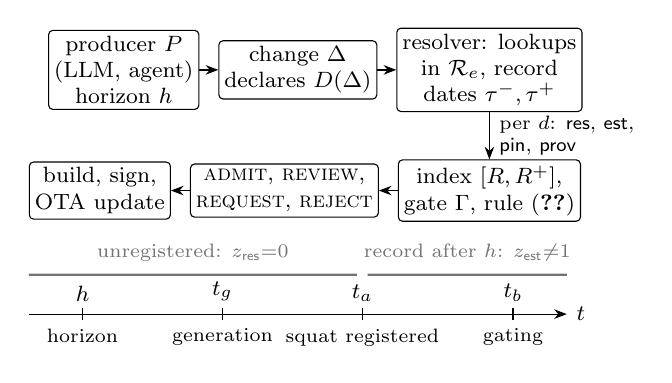
\begin{tikzpicture}[font=\footnotesize, node distance=3mm and 2.4mm,
  box/.style={draw, rounded corners=1.5pt, align=center, inner sep=2pt, minimum height=6mm, fill=white},
  arr/.style={-{Stealth[length=1.6mm]}, semithick}]
\node[box] (p) {producer $P$\\ (LLM, agent)\\ horizon $h$};
\node[box, right=of p] (m) {change $\Delta$\\ declares $D(\Delta)$};
\node[box, right=of m] (r) {resolver: lookups\\ in $\Reg_e$, record\\ dates $\tau^-,\tau^+$};
\node[box, below=6mm of r] (g) {index $[R,R^{+}]$,\\ gate $\Gamma$, rule (\ref{eq:rule})};
\node[box, left=of g] (o) {\dec{admit}, \dec{review},\\ \dec{request}, \dec{reject}};
\node[box, left=of o] (b) {build, sign,\\ OTA update};
\draw[arr] (p) -- (m); \draw[arr] (m) -- (r);
\draw[arr] (r) -- node[right, font=\scriptsize, align=left] {per $d$: $\sres$, $\sest$,\\ $\spin$, $\sprov$} (g);
\draw[arr] (g) -- (o); \draw[arr] (o) -- (b);
\coordinate (L) at ($(b.south west)+(0,-12mm)$);
\coordinate (Q) at ($(r.east |- L)+(-2mm,0)$);
\draw[-{Stealth[length=1.6mm]}] (L) -- (Q) node[right] {$t$};
\foreach \f/\l/\s in {0.10/h/horizon, 0.36/{t_g}/generation, 0.62/{t_a}/{squat registered}, 0.90/{t_b}/gating}{
  \coordinate (T) at ($(L)!\f!(Q)$);
  \draw ($(T)+(0,0.08)$) -- ($(T)+(0,-0.08)$); \node[above] at ($(T)+(0,0.04)$) {$\l$};
  \node[below, font=\scriptsize] at ($(T)+(0,-0.06)$) {\s};}
\draw[thick, black!55] ($(L)+(0,0.5)$) -- ($($(L)!0.61!(Q)$)+(0,0.5)$) node[midway, above=1pt, font=\scriptsize] {unregistered: $z_{\sres}{=}0$};
\draw[thick, black!55] ($($(L)!0.63!(Q)$)+(0,0.5)$) -- ($(Q)+(0,0.5)$) node[midway, above=1pt, font=\scriptsize] {record after $h$: $z_{\sest}{\ne}1$};
\end{tikzpicture}
\caption{Gating AI-originated dependency declarations. Bottom: whatever the gating time, a phantom is never admitted:
before the squat it does not resolve; after it, its establishment is refuted where the registry dates record
creation, and undecided, held for evidence, where it bounds it from above only.}
\label{fig:pipeline}
\end{figure}

% =====================================================================
\section{Horizon-Anchored Evidence for Dependencies}
\label{sec:approach}

\subsection{Evidence for one dependency}
For each dependency $d\in D(\Delta)$ that a change declares, the gate collects four evidence items, each in one of
three states: confirmed ($1$), refuted ($0$) or absent ($\bot$). Absent means that no evidence was obtained (not
produced, not reachable, or not decidable); refuted means that evidence contradicts the requirement. The first two
items are mandatory:
\begin{itemize}
\item $\sres$ (resolution): $1$ if $d$ resolves in $\Reg_e$ at gating time or is provided by the toolchain; $0$ if the
registry is authoritative for the name and it does not resolve; $\bot$ if resolution cannot be decided (a VCS URL, a
path, a legacy numeric identifier, a failed lookup, a package outside the snapshots). A name resolves only as the
installer resolves it: PyPI names after its normalisation, PlatformIO and ESP names up to case as their APIs match
them, all other names exactly (Cargo, for one, rejects a crate written with \texttt{\_} for \texttt{-} or in another
case); a PyPI project without files and a crate whose versions are all yanked do not resolve, because the installer
finds nothing to install. A registry match takes
precedence over the toolchain list.
\item $\sest$ (establishment): with a lower bound $\tau^{-}$ and an upper bound $\tau^{+}$ on the first publication
time $\tau(d)$, horizon $h$ and margin $\delta\ge 0$,
\begin{equation}
z_{\sest}=\begin{cases} 1 & \tau^{+}\le h-\delta,\\ 0 & \tau^{-}>h,\\ \bot & \text{otherwise (including unknown bounds).}\end{cases}
\label{eq:est}
\end{equation}
\item $\spin$ (content pinning): $1$ if the pipeline records a digest of the resolved artifact in a lock file (or the
declaration pins a full commit hash), $0$ on a digest mismatch, $\bot$ otherwise.
\item $\sprov$ (publisher provenance): $1$ if provenance is present and valid, $0$ if verification fails,
$\bot$ if absent.
\end{itemize}
The margin $\delta$ keeps records created just before the horizon undecided: a model can hardly have learned a
package from the last weeks of its training data. The bounds come from the registry and describe the record. Where the
registry dates the creation of the record (PlatformIO \texttt{added\_at}, ESP \texttt{created\_at}, the crates.io
\texttt{pubtime} of the first version, npm \texttt{time.created}), both bounds equal that time. PyPI reports only the
upload times of files that still exist: the earliest bounds the record from above and is no lower bound, because
earlier files may have been deleted. The Arduino Library Manager and the ROS distribution keep their registries in git,
and their indices carry no dates; we date a library or a package by the first change on the main line of the registry
repository that added it (a pull-request merge that GitHub creates, or a maintainer's commit), so the date is set by the
registry and not by the submitter. Arduino moves are linked where the log shows them, and libraries of the initial
import get an upper bound only. ROS packages are dated in the distribution file of the release the tasks name
(Humble). MicroPython packages get an upper bound from the first commit to their manifest in micropython-lib by a
maintainer; commits by other committers carry dates a contributor chose. An owner-less PlatformIO name may install
any same-name package, so its bounds span all candidates and stay undecided if one candidate has no date. A pipeline
that looked a name up and found it unregistered holds a further lower bound, its \emph{absence record}, for any record
that appears later. Toolchain-provided names inherit the evidence of the platform and are confirmed.

\subsection{From a manifest to a decision}
The gate $\Gamma$ of a change is $0$ if some item of some declaration is refuted, $\bot$ if none is but a mandatory
item is absent, and $1$ otherwise. Once the gate passes, a graded index decides between \dec{admit} and \dec{review}:
it encodes the optional evidence a project demands before a change goes in unreviewed. With item weights
$\alpha_s\ge 0$ that sum to $1$ and a threshold $\theta\in(0,1]$, the lower and upper labels of a declaration count
absent items as failed and as confirmed, respectively,
\begin{equation}
\ell(d)=\sum_{s}\alpha_s[z_s(d)=1],\qquad \ell^{+}(d)=\sum_{s}\alpha_s[z_s(d)\neq 0],
\label{eq:labels}
\end{equation}
and the index of the change is $R=\prod_{d}\ell(d)$, with $R^{+}=\prod_{d}\ell^{+}(d)$; any completion of the absent
items yields an index in $[R,R^{+}]$. The decision is
\begin{equation}
\Dec(\Delta)=\begin{cases}
\dec{reject} & \Gamma=0 \ \text{or}\ (\Gamma=1 \wedge R^{+}<\theta),\\
\dec{request} & \Gamma=\bot,\\
\dec{admit} & \Gamma=1 \wedge R\ge\theta,\\
\dec{review} & \text{otherwise}.
\end{cases}
\label{eq:rule}
\end{equation}
The gate is non-compensable: no weight can offset a refutation, and a missing mandatory item is reported instead of
being scored. Rejects and requests come from the gate, reviews from the index. With this gate, $\Gamma=1$ implies that
no item is refuted, hence $R^{+}=1\ge\theta$; the $R^{+}$ clause matters only for the index-only variant below, and we
keep the rule in the form of~\cite{anon2026evidence}.

\emph{General form.} The index is the supply-chain integrity index (SCII) of~\cite{anon2026evidence} for one release
step; we restate what this paper uses and prove the properties it relies on, so nothing below depends on that work. A
profile $\Prof=(V,E,w,S,S^{*},\alpha,\theta)$ fixes a directed acyclic graph of process vertices whose root $\rho$ is
the release, edge weights $w_{uv}\in[0,1]$ on edges $u\to v$ from a supplying to a consuming vertex, and for each
vertex $v$ the items $S_v$ it expects, with weights summing to $1$, and the mandatory subset $S^{*}_v\subseteq S_v$.
Labels (\ref{eq:labels}) are computed per vertex, so $\ell(d)$ is the label of the vertex $v_d$ of declaration $d$,
with $\ell(v)=\ell^{+}(v)=1$ for a vertex without items, and propagate with a product kernel,
\begin{equation}
r(v)=\ell(v)\prod_{(u,v)\in E}\bigl(1-w_{uv}\,(1-r(u))\bigr),
\label{eq:index}
\end{equation}
giving $R=r(\rho)$ and, with $\ell^{+}$ for $\ell$, $R^{+}$. A change instantiates the graph with one vertex $v_d$
per declaration and an edge of weight $1$ into the dependency-resolution vertex, because a compromised dependency
compromises the build; that vertex carries no evidence of its own and is the root of the part of the graph that
changes, so (\ref{eq:index}) reduces to the products above.

\subsection{Properties}
\begin{proposition}[Non-compensability]
If $z_{\sres}(d)=0$ for some $d\in D(\Delta)$, then $\Dec(\Delta)=\dec{reject}$ for every $\alpha$ and $\theta$.
\end{proposition}
\begin{IEEEproof}
A refuted item sets $\Gamma=0$, and (\ref{eq:rule}) rejects whenever $\Gamma=0$.
\end{IEEEproof}

\begin{proposition}[Horizon soundness]
Let $P$ declare $d$, where $d$ is neither provided by the toolchain nor declared in $\Delta$, and no package of that
name, as the installer resolves it, was registered in $\Reg_e$ at any time $t\le h(P)$. Assume that every upper
bound the resolver reports is valid within the margin, $\tau^{+}\ge\tau(d)-\delta$, where $\tau(d)$ is the
first publication of the package the installer would fetch. Then, with $\sres$ and $\sest$ mandatory, for every gating
time $t_b$, every registry state at $t_b$, and every $\alpha,\theta$, $\Dec(\Delta)\neq\dec{admit}$.
\end{proposition}
\begin{IEEEproof}
If $d$ does not resolve at $t_b$, then $z_{\sres}=0$, or $z_{\sres}=\bot$ if the lookup fails. Otherwise the package it
resolves to was first published at $\tau(d)>h$, so $\tau^{+}\ge\tau(d)-\delta>h-\delta$, or $\tau^{+}$ is unknown, and
(\ref{eq:est}) gives $z_{\sest}\neq 1$. In every case a mandatory item is refuted or absent, so $\Gamma\in\{0,\bot\}$
and the decision is \dec{reject} or \dec{request}.
\end{IEEEproof}
The two baselines behave differently. A resolves-now check admits $d$ from the moment of registration; an age rule with
threshold $N$ admits it $N$ days later. Proposition~2 holds at every $t_b$ because $h$ does not move, and it covers a
post-horizon match, whatever the reason the model wrote its name. Its guarantee starts at the horizon the gate uses:
an upper bound on the true cut-off leaves registrations between the two unprotected (Section~\ref{sec:threat}), a
further reason to keep the bound tight. The margin also absorbs small offsets between the date a registry records and the time it serves a
package, such as the delay between a merge and the next index build. Correct lower bounds matter only for
refutations; an invalid $\tau^{-}$ can turn \dec{request} into \dec{reject}, never into \dec{admit}.

\emph{Scope.} The guarantee is exactly this: a name whose record is first created after $h$ is never admitted, when
record dates are valid within $\delta$ and the registry is not compromised. It says nothing about a package that
already existed at $h$ (a classic typosquat or a malicious old package), a new \emph{version} of such a package
(content pinning and provenance, the optional items, bear on that), or a compromised publisher. It ranges over the
declarations the model wrote, not over the transitive closure the installer resolves later: the horizon says nothing
about packages the model never named, which other evidence, such as pins in the lock file, has to cover.

\begin{proposition}[Monotone confirmation]
Replacing an absent item by a confirmed one never decreases $R$ or $R^{+}$, and never turns \dec{admit} into another
decision.
\end{proposition}
\begin{IEEEproof}
By (\ref{eq:labels}), $\ell$ grows by $\alpha_s\ge 0$ and $\ell^{+}$ is unchanged. The kernel in (\ref{eq:index}),
and the product it reduces to, is non-decreasing in every $r(u)$ and in $\ell(v)$, so $R$ does not decrease and $R^{+}$
is unchanged. \dec{admit} requires
$\Gamma=1$ and $R\ge\theta$; confirming an item cannot create a refutation or an absent mandatory item, so both conditions
persist.
\end{IEEEproof}

\begin{proposition}[Insufficiency of the index alone]
The index-only rule (``\dec{reject} if $R^{+}<\theta$, \dec{admit} if $R\ge\theta$, else \dec{review}'') admits a
squatted dependency for some admissible $\alpha,\theta$.
\end{proposition}
\begin{IEEEproof}
Take $\alpha=(0.5,0.05,0.4,0.05)$ for $(\sres,\sest,\spin,\sprov)$ and $\theta=0.85$. A squatted name resolves
($z_{\sres}=1$), the pipeline pins whatever it resolved ($z_{\spin}=1$), $z_{\sest}=0$ and $z_{\sprov}=\bot$. Then
$\ell=0.9\ge\theta$ and the index-only rule admits it, while (\ref{eq:rule}) rejects because $\Gamma=0$.
\end{IEEEproof}
Exactly: a squat has $z_{\sest}\neq 1$ and $z_{\sprov}=\bot$, so its label is $\alpha_{\sres}+\alpha_{\spin}$ if
pinned and $\alpha_{\sres}$ if not, and the index-only rule can admit a manifest containing it only if
$\alpha_{\sest}+\alpha_{\sprov}\le 1-\theta$, or $\alpha_{\sres}\ge\theta$ without a pin; Section~\ref{sec:rq3} samples
how often profiles satisfy this. A rule that rejects whenever $z_{\sest}\neq 1$ would also be safe, but it rejects
every change whose record dates are missing or one-sided.

\emph{Relation to date filters.} Consider a filter on the record-creation time at $h$: it admits a record known to
predate $h$ and hides a later one. Give it a third answer, \emph{unknown}, for a record it cannot place, and let it ask
for evidence then: this filter (P3$_\bot$ in Section~\ref{sec:gateeval}) is exactly the gate. With
$\alpha_{\spin}=\alpha_{\sprov}=0$, $\delta=0$ and no optional item refuted (P3$_\bot$ ignores pins and
provenance), rule~(\ref{eq:rule}) decides every change as P3$_\bot$ does, since $\Gamma=1$ then implies $R=1$; the
analysis checks this on every manifest and world, and a unit test on random dependency sets. The comparison is to
this record-age filter, not to the installers' upload- or version-time filters
(Section~\ref{sec:gateeval}). The graded index adds what blocking does not need: optional evidence (pinning,
provenance) that decides between \dec{admit} and \dec{review}, and the margin $\delta$.

\emph{Cost.} The index and gate take one pass over the change, $O(|D(\Delta)|)$ here and $O(|V|+|E|)$ in general;
registry lookups dominate and are cached.

\subsection{Implementation}
\textsc{PhantomDeps-CPS} (Python) renders prompts, queries OpenAI-compatible endpoints, classifies declarations
against snapshots and cached registry answers, evaluates the policies and writes every number of this paper with a
provenance tag. Unit tests check Propositions~1--4 on random
profiles and through the pipeline, the equivalence with P3$_\bot$ on 4{,}000 random dependency sets, registry-history
dating and the extraction rules. The analysis aborts if the rule admits a squat, if the classification came from
other code or snapshots, or if the data contradict one of the statements of Section~\ref{sec:results} that it
checks, such as that every policy but P0 rejects every manifest with a phantom.

% =====================================================================
\section{Study Design}
\label{sec:design}

We ask four research questions.
\textbf{RQ1} (prevalence): how often do code models declare phantom dependencies when they produce build manifests for
CPS ecosystems, and how does this vary by ecosystem, model, task tier, prompt family and answer quality?
\textbf{RQ2} (exposure): do phantoms recur across models and runs, do suggested names already resolve to records
created after the model's horizon, and which phantoms could an outsider register?
\textbf{RQ3} (gating): how do baseline policies, date filters and the horizon-anchored rule decide on the generated
manifests, in the observed registry state and when phantoms are squatted, and what do they cost in availability?
\textbf{RQ4} (evidence and cost): how often can establishment be decided, what lock files and provenance do the tools
supply, and what does gating cost?
The protocol was fixed before the study run; its change log lists every later change and why it was made.

\subsection{Ecosystems and snapshots}
Table~\ref{tab:registries} lists the eight ecosystems: the firmware layer (Arduino, PlatformIO, ESP-IDF, embedded
Rust, MicroPython), robotics (ROS~2) and the gateway layer of industrial systems (PyPI, Node-RED nodes on npm). Static
indices (Arduino and MicroPython indices, the \texttt{humble} and \texttt{jazzy} distribution files, the
\texttt{rosdep} databases) were downloaded and hashed, and the registry repositories of Arduino, ROS and MicroPython
cloned at recorded commits; other registries were queried per name, with every answer cached with its retrieval time
(latest: \rSnapshotDate). Toolchain names come from nine Arduino cores, the ESP-IDF components (v5.5 and master), the
MicroPython documentation and the Python standard library, matched up to case and separators (which can only
lower phantom counts).

\begin{table}[t]
\centering
\caption{Ecosystems: how a name enters the registry, source of the record-date bounds, digest locking, resolved
declarations with a decidable $\sest$, and decisions of rule (\ref{eq:rule}) on clean manifests
(Section~\ref{sec:gateeval}) per task ecosystem (A admit, ? review or request, X reject).}
\label{tab:registries}
\footnotesize
\setlength{\tabcolsep}{2.5pt}
\begin{tabular}{@{}lllcrr@{}}
\toprule
Ecosystem & New names & Dates & Lock & $\sest$ decided & $C$: A/?/X \\
\midrule
Arduino LM & open, automated & merge log & no & 357/359 & 0/95/0 \\
PlatformIO & open, owner ns. & API & no & 338/393 & 0/80/0 \\
ESP-IDF & open, namespace & API & yes & 35/37 & 2/14/0 \\
ROS~2 & PR review & merge log & no & 1795/1796 & 0/68/0 \\
crates.io & open & index & yes & 1439/1440 & 1/108/0 \\
MicroPython & PR review & git (upper) & no & 93/93 & 14/47/0 \\
PyPI & open & files (upper) & yes & 657/680 & 36/165/0 \\
npm & open, name rules & API & yes & 345/345 & 40/67/0 \\
\bottomrule
\end{tabular}

\end{table}

\subsection{Task corpus}
The corpus has \rNTasks{} tasks, \rTasksPerEco{} per ecosystem (SHA-256 prefix \texttt{\rCorpusSha}). Each task names a board or
host and a function in one of eleven categories (sensing, actuation, IoT, fieldbus, positioning, security, control,
data, display, wireless, robotics), but no package, so the dependency names are chosen by the model. In ROS, two
tasks name a standard message type and thus its package, and a few name the framework that defines the interface.
Half the tasks of each ecosystem went to a \emph{common} tier (well-documented devices and protocols, such as
a BME280 sensor or MQTT) and half to a \emph{niche} tier (less common fieldbuses such as J1939, DNP3 or IEC~61850,
secure-update functions, specific GNSS or IMU parts) before any generation. Two prompt families wrap each task: F1
asks for the manifest and the source code, F2 for the manifest or install commands only. For example, the F2 prompt of
task \texttt{platformio-07} reads: \emph{``Create a PlatformIO project for an ESP32-S3 DevKitC using the Arduino
framework. Task: Poll holding registers of a PLC over Modbus TCP and forward the values to MQTT. Provide only the
complete platformio.ini, including lib\_deps. Do not write the source code.''} All prompts share one system message
(in the artifact).

\subsection{Models and generation}
\label{sec:models}
\ifpilot
The study configuration covers \rStudyNModels{} open-weight models from \rStudyNVendors{} vendors, \rStudyMinParams{}
to \rStudyMaxParams{} billion parameters, whose repositories were created from \rStudyFirstHorizon{} to
\rStudyLastHorizon{} (horizons will be anchored to the hub files that are run, as in the pilot), served by Ollama one
request at a time. Each prompt of both families receives one greedy answer (temperature \rStudyGreedyTemp, fixed seed) under
one token budget for both families. Every (model, prompt) pair whose greedy answer contains a
phantom is asked \rStudyResampleN{} more times at temperature \rStudyResampleTemp{} to measure persistence. Reasoning
models get a larger budget and only their final answer is analysed; the runner records the served model digest.
The pilot reported in this version (Table~\ref{tab:models}) runs \rNModels{} models of \rRunMinParams--\rRunMaxParams B
parameters through llama.cpp~\cite{llamacpp} on two vCPUs, with greedy decoding (seed \rGenSeed, repeat penalty
\rRepeatPenalty): three small ones from the Qwen2.5-Coder~\cite{hui2024qwen25coder}, DeepSeek-Coder~\cite{guo2024deepseekcoder}
and Llama~3~\cite{grattafiori2024llama3} families with a budget of \rBudgetMin{} tokens for F2\ifnum\rHasFamCmp=1{}
(and \rMaxTokFOne{} for F1, which \rFOneModels{} also answered)\fi, and \rResampleN{} resamples per phantom-producing
pair\ifnum\rHasGroups=1; and \rGrpLargeN{} larger ones (Llama~3.2 3B and Qwen2.5-Coder 7B of the same families,
Phi-3-mini 3.8B~\cite{abdin2024phi3} of a fourth vendor) with a budget of \rBudgetMax{} tokens for F2, raised so
that answers finish\fi.
\ifnum\rNRemovedModels=1 Another, \rRemovedModel, was stopped by the host's time limit after \rRemovedAnswers{} of
\rNTasks{} answers and is not analysed. \fi
\ifnum\rHasFamEq=1 A separate run asks \rFamEqModel{} both families under one budget of \rFamEqBudget{} tokens on
\rFamEqTasks{} tasks; it enters only the family comparison. \fi
\else
The study ran \rNModels{} open-weight models from \rStudyNVendors{} vendors, \rRunMinParams{} to \rRunMaxParams{}
billion parameters (Table~\ref{tab:models}): Qwen2.5-Coder~\cite{hui2024qwen25coder}, Llama~3.1 and
3.2~\cite{grattafiori2024llama3}, DeepSeek-Coder~\cite{guo2024deepseekcoder} and its V2~\cite{deepseek2024coderv2},
Granite~3.3~\cite{granite33}, Gemma~3~\cite{gemmateam2025gemma3}, Phi-4~\cite{abdin2024phi4}, and the reasoning
models Qwen3~\cite{yang2025qwen3} and gpt-oss~\cite{openai2025gptoss}. Each model is the hub GGUF file we pinned by
its SHA-256, quantised as the Ollama library's default, and was served by Ollama~\rOllamaVersion{} with the library's
chat template and default parameters (our system message replaces a library default), one request at a time, with
an 8{,}192-token context on a laptop GPU with 12~GB (the two largest models partly in system memory). Each prompt of both families received one greedy answer (seed \rGenSeed) under one budget of
\rBudgetMin{} tokens for both families; the reasoning models got \rBudgetMax{} tokens, and only their final answer is
analysed. Every (model, prompt) pair whose greedy answer contained a phantom was asked \rResampleN{} more times at
temperature \rResampleTemp{} to measure persistence\ifnum\rHasExt=1, and every cut answer was generated again with
\rExtBudget{} tokens as a sensitivity analysis\fi. A pilot with smaller models on a CPU host had validated the harness
beforehand; the artifact holds it.
\fi
Primary metrics use the prompt families answered by every model (\rFamilies), so that every model contributes the same
prompts. The horizon of each model is the date at which its weights demonstrably existed (Section~\ref{sec:threat}),
read from the commit history of the model hub; it lies within \rHorizonGapMaxH{} hours of the creation of each
repository, and the files we ran, identified by SHA-256, were committed \ifnum\rNGgufIsHorizon>0 \rGgufGapLaterMinD{} to
\rGgufGapMaxD{} days later (for \rNGgufIsHorizon{} model, whose vendor weights changed afterwards, the commit of the
file we ran is the horizon)\else\rGgufGapMinD{} to \rGgufGapMaxD{} days later\fi.

\begin{table}[t]
\centering
\caption{\ifpilot Pilot models (primary family)\else Models (primary families)\fi: horizon $h$, token budget, answers
cut by it, and yield (answers with an executable declaration); Table~\ref{tab:prevalence} gives their phantom rates.}
\label{tab:models}
\footnotesize
\setlength{\tabcolsep}{4pt}
\begin{tabular}{@{}lrrrr@{}}
\toprule
Model & Horizon $h$ & Budget & Cut & Yield \\
\midrule
Qwen2.5-C 1.5B & 2024-09-18 & 1536 & 85 & 167/192 \\
Llama-3.2 3B & 2024-09-18 & 1536 & 60 & 134/192 \\
Qwen2.5-C 7B & 2024-09-17 & 1536 & 24 & 183/192 \\
DS-Coder 6.7B & 2023-10-29 & 1536 & 15 & 168/192 \\
Llama-3.1 8B & 2024-07-18 & 1536 & 51 & 152/192 \\
Qwen3 8B & 2025-04-28 & 4096 & 34 & 153/192 \\
Granite-3.3 8B & 2025-04-09 & 1536 & 11 & 152/192 \\
Gemma-3 12B & 2025-03-12 & 1536 & 107 & 166/192 \\
Qwen2.5-C 14B & 2024-11-06 & 1536 & 25 & 164/192 \\
Phi-4 14B & 2024-12-11 & 1536 & 9 & 164/192 \\
DS-Coder-V2 16B & 2024-06-14 & 1536 & 21 & 188/192 \\
gpt-oss 20B & 2025-08-04 & 4096 & 102 & 107/192 \\
Qwen2.5-C 32B & 2024-11-10 & 1536 & 18 & 185/192 \\
\bottomrule
\end{tabular}

\end{table}

\subsection{Extraction and classification}
\label{sec:extraction}
Only executable declarations are extracted: manifest entries (\texttt{lib\_deps}, \texttt{idf\_component.yml},
\texttt{package.xml}, \texttt{Cargo.toml}, requirement lists, \texttt{package.json}, \texttt{library.properties})
and install commands (\texttt{arduino-cli}, \texttt{pio}, \texttt{idf.py}, \texttt{cargo add}, \texttt{mip},
\texttt{pip}, \texttt{npm}, \texttt{apt} for ROS packages) in code context, with arguments ending at the first token
that reads as prose. ESP-IDF manifests that list dependencies instead of mapping them are extracted and flagged, since
a developer would fix the syntax and keep the names. Prose recommendations are ignored, so the counts are lower bounds
on what a reader would try to install. The ecosystem of a declaration follows from its syntax. A declaration is classified as \emph{exists}, \emph{phantom}, \emph{toolchain}, \emph{local} (a ROS
package of the same workspace), \emph{non-registry} (URL or path), \emph{legacy identifier}, \emph{special} (not a
package, such as the ESP-IDF version constraint), \emph{unsupported} (a package outside the snapshots, such as one of
another ROS distribution; gated with undecided resolution) or \emph{unresolved} (lookup failure).

To separate answer quality from hallucination, every manifest file is parsed independently of the extractor with the
parser of its ecosystem's tooling (\texttt{tomllib}, JSON, \texttt{packaging}, \texttt{configparser},
\texttt{catkin\_pkg}, the component manager's YAML schema); answers count as well-formed, malformed, commands only or
cut by the token limit, and on well-formed files the extractor's names are compared with the parsers'.
\ifnum\rHasValidation=0 The protocol's manual validation, 200 answers labelled by two annotators, is still to be
done for this version.\fi

\subsection{Gate evaluation}
\label{sec:gateeval}
A manifest is the set of non-local, non-special declarations in one response. It is \emph{unsafe} ($U$) if it contains
a phantom, \emph{post-horizon} ($H$) if it contains a post-horizon match but no phantom, and \emph{clean} ($C$)
otherwise. \emph{Clean} means only that our lookups found no phantom and no post-horizon match; such a manifest need
not build (it may name a version that does not exist) and is not certified safe. We compare nine policies:
P0 admits everything;
P1 (resolves now) rejects a manifest with a declaration known not to resolve and lets URLs, paths and failed lookups
pass, as an installation would;
P2 adds an age rule: every package with a known date must be at least \rAgeDays{} days old;
P3 counts a registry package only if its registry \emph{record} is known to have been created by $h$, treats a record
without a date as unavailable, and does not date-filter URLs, paths and failed lookups;
P3$_\bot$ is P3 with a third answer: it rejects what is known to be newer than $h$, admits what is known to be older,
and requests evidence for everything else, URLs and paths included;
I is the index-only rule; T (two-state) reads an absent mandatory item as refuted; O (optimistic) reads every absent
item as confirmed; and SCII is rule~(\ref{eq:rule}). P3 is an abstract \emph{record-age} policy: it tests what a
squat changes, a new record under an old-looking name. The installers' filters test something else: uv
\texttt{--exclude-newer} filters distribution \emph{upload} times and npm \texttt{before} \emph{version} publish
times, which decide the version that installs (a 2020 package with a 2026 release passes P3 but loses that release
under the filters). They coincide with P3 only when a name's earliest artifact dates its record, so we use them in
the replay (Section~\ref{sec:replay}) and P3 in the evaluation.
The profile is assigned, not fitted:
$\alpha=(\rAlphaRes,\rAlphaEst,\rAlphaPin,\rAlphaProv)$, $\theta=\rTheta$, $\delta=\rDeltaDays$ days. No publisher
provenance is evaluated, so $\sprov=\bot$ for every registry package.

We evaluate three worlds. In the \emph{observed} world, registry state is the snapshot and
\ifnum\rMainLock=1 $\spin=1$ only where the lock file that the ecosystem's own tool wrote for the answer records a
digest for the declaration (Cargo, npm and uv, Section~\ref{sec:rq4}); other declarations are unpinned. For
comparison we also decide with the capability alone, $\spin=1$ wherever the tooling can lock digests
(Table~\ref{tab:registries}). \else $\spin=1$ where the ecosystem's tooling locks digests
(Table~\ref{tab:registries}). \fi In the \emph{squat} world, every phantom is registered by the adversary one
day after the snapshot, without provenance but pinned wherever the tooling can lock (the worst case for blocking),
and the gate runs $L$ days later; registered names without installable files stay with their owners. The evidence of a squat follows the
resolver of its ecosystem: a refuted $\sest$ where the registry dates the creation of records, absent where it bounds
them from above only (PyPI, MicroPython); the gate meets the name for the first time after the squat, and a variant
gives it the absence record of our snapshot lookup. The \emph{open squat} world registers only phantoms that any
account holder could register. To see what registry histories contribute, we also decide every manifest without the
dates derived from them (Arduino, ROS, MicroPython), as a filter that reads only the installers' indices would. The
sweep draws \rSweepN{} profiles with $\alpha\sim\mathrm{Dirichlet}(1,1,1,1)$ and
$\theta\sim U(\rSweepThetaMin,\rSweepThetaMax)$, and a grid over $\theta$ and $\alpha_{\sprov}$ (the other weights
keep their ratios) measures availability on clean manifests.
\ifnum\rHasReplay=1
Finally, we replay squats against real installers (pip, uv, npm, Cargo) and registries on the local host, and build
an ESP-IDF application that declares a stand-in for one (Section~\ref{sec:replay}).
\fi

\subsection{Statistics and ethics}
Rates come with 95\% percentile bootstrap intervals (\rBootB{} replicates, seed \rSeed) that resample tasks, because
the answers of all models to one task, and the declarations within one answer, are not
independent~\cite{field2007bootstrap}; persistence resamples (model, prompt) pairs. Cells with fewer than ten registry
declarations or from a single task are reported but not interpreted. Nothing was published to a public registry, no
package code ran outside the replay (local registries, harmless packages), lookups were read-only and cached, and
lock files were written in resolve-only modes. Names an outsider may be able to register appear as keyed pseudonyms
and will be reported to the registry operators before publication; a name that is also a real package elsewhere
stays readable there.

% =====================================================================
\section{Results}
\label{sec:results}

The reported configuration produced \rNGen{} responses in the primary families (\rNTrunc{} hit the token limit).
Of these, \rNRespDecl{} (\rYield) contained at least one executable declaration, for \rNDecl{} declarations in total:
\rNExists{} exist, \rNPhantom{} are phantoms, \rNToolchain{} are toolchain names, and \rNOtherDecl{} fall in the
other classes of Section~\ref{sec:extraction}. Of the \rNRespNoDecl{} responses without a declaration, \rNRespNoBlock{} contained no code block at all. The
answers contained \rNFiles{} manifest files, of which the ecosystems' own parsers rejected \rNFilesMalformed{}
(\rFilesXmlBad{} of \rFilesXml{} \texttt{package.xml}, \rFilesIdfBad{} of \rFilesIdf{} \texttt{idf\_component.yml},
\rFilesCargoBad{} of \rFilesCargo{} \texttt{Cargo.toml}, \rFilesPioBad{} of \rFilesPio{} \texttt{platformio.ini},
\rFilesReqBad{} of \rFilesReq{} requirement lists); \rNMalformed{} registry declarations (\rNMalformedPhantom{} of them
phantoms) come from malformed ESP-IDF manifests. On the well-formed files, the extractor declared \rOffTp{} of the
names the official parsers found, missed \rOffFn{} and added \rOffFp{} (precision \rOffPrecision, recall
\rOffRecall{} against the tools' own reading; both find requirement lists with the same rule, so recall on them is an
upper bound). \ifpilot The check found one gap, which the extractor now closes: requirement lists in code blocks
labelled as Python or shell that the text right before them calls requirements.\else The check and \rNPrescreenWord{} LLM
pre-screens of \rPrescreenEach{} answers each (not counted as validation) found extraction errors that the extractor now
handles (comments, unfenced requirement lists, MicroPython's \texttt{upip}, irregular ESP-IDF manifests); the manual
validation uses a fresh sample.\fi
\ifnum\rHasValidation=1{} \ifnum\rValAllIdentical=1 Two annotators from one university group labelled a stratified
sample of \rValN{} responses jointly; against their labels\else Two annotators labelled a stratified sample of \rValN{}
responses; against the first\fi, extraction had a precision of \rValPrecision{} (CI \rValPrecisionCI) and a recall
of \rValRecall{} (CI \rValRecallCI). \ifnum\rValSpurNonreg=\rValSpur\relax All \rValSpur\else\rValSpurNonreg{} of
\rValSpur\fi{} spurious and \rValMissNonreg{} missed items are dependencies by URL that the extractor names by package,
the annotators by URL; \rValMissTop{} of the \rValMissed{} missed items are tables of one \texttt{Cargo.toml} that does
not parse. The errors cluster in few responses\ifnum\rValByResponse=1, so the intervals resample responses\fi: extraction
was exact on \rValRespExact{} of \rValN{} (\rValRespExactPct, Wilson CI \rValRespExactCI), with a miss in
\rValRespMissed{} and a spurious item in \rValRespSpur.\ifnum\rHasKappa=1\ifnum\rValAllIdentical=0{} The two annotators
agreed on whether extraction was exact with Cohen's $\kappa=\rValKappa$.\fi\fi{} This step validates extraction, not
the phantom/exists/toolchain classification,
which rests on the registry lookups and name rules of Section~\ref{sec:extraction}; an independent double annotation of
both is future work.
\fi

\subsection{RQ1: prevalence}
\label{sec:rq1}
Of \rDeclRegistry{} registry declarations, \rDeclPhantom{} were phantoms (\rPhantomDecl, 95\% CI \rPhantomDeclCI).
At the response level, \rRespK{} of \rRespN{} responses with a registry declaration contained a phantom
(\rPhantomResp, CI \rPhantomRespCI). The pooled rate weights models by how much they declare: \rTopModel{} contributed
\rTopModelShare{} of the registry declarations, and the mean of the per-model rates is \rMacroPhantom.
\ifnum\rHasGroups=1
The \rGrpSmallN{} small models (\rGrpSmallMinB--\rGrpSmallMaxB B, budget \rBudgetMin{} tokens) hit the token limit in
\rGrpSmallTrunc{} of their answers and declared phantoms at \rGrpSmallDecl{} (\rGrpSmallK/\rGrpSmallDeclN, CI
\rGrpSmallDeclCI); the \rGrpLargeN{} larger ones (\rGrpLargeMinB--\rGrpLargeMaxB B, budget \rBudgetMax) hit it in
\rGrpLargeTrunc{} and declared phantoms at \rGrpLargeDecl{} (\rGrpLargeK/\rGrpLargeDeclN, CI \rGrpLargeDeclCI).
Without the cut answers the two rates are \rGrpSmallDeclNoTrunc{} and \rGrpLargeDeclNoTrunc; per answer, a phantom
appeared in \rGrpSmallResp{} (\rGrpSmallRespK/\rGrpSmallRespN) and \rGrpLargeResp{} (\rGrpLargeRespK/\rGrpLargeRespN) of
the answers with a registry declaration.
\fi
\ifnum\rMaxAnsCut=1 Declaration counts are sensitive to repetition loops: the largest single answer, cut by the limit,
held \rMaxAnsDecl{} registry declarations, \rMaxAnsPhantom{} of them phantoms (\rMaxAnsModel). \fi
Table~\ref{tab:prevalence} breaks the rate down.
\ifnum\rNEcoTen>1
Among the \rNEcoTen{} ecosystems with at least ten registry declarations, the highest rate was in \rMaxEco{}
(\rMaxEcoRate) and the lowest in \rMinEco{} (\rMinEcoRate). Common-tier tasks yielded \rPhantomCommon{}
(\rPhantomCommonK/\rPhantomCommonN, CI \rPhantomCommonCI) and niche tasks \rPhantomNiche{}
(\rPhantomNicheK/\rPhantomNicheN, CI \rPhantomNicheCI).
\fi
Answer quality matters, and the subsets answer different questions (Table~\ref{tab:subset}): the \rPhantomDecl{}
over all declarations falls to \rPhantomDeclNoTrunc{} on finished answers and to \rRateWellformed{} on finished answers
whose manifests all parse, so the headline \rPhantomResp{} of answers is not a count of exploitable builds. Repeats do
not inflate the rates: the extractor counts each name once per answer, and repetition loops produce distinct names.
By ecosystem the quality effect is uneven (Table~\ref{tab:subset}, bottom): ESP-IDF, highest overall at \rMaxEcoRate,
is \rWfEspP{} (\rWfEspK/\rWfEspN) on well-formed complete answers, the rest coming from manifests the component manager
cannot read. Arduino, MicroPython and npm packages were declared only in install commands, so that subset holds none of
them and its rate covers the other five ecosystems.
\ifnum\rCutText>0

\emph{Cut answers.} \rNTrunc{} answers (\rTruncPct) reached the budget; of the \rCutText{} with a final text, \rCutLoop{}
ended in a repetition loop (their last \rLoopChars{} characters compress below \rLoopZlib{} of their size). Without the cut
answers, \rPhantomRespNoTrunc{} (CI \rPhantomRespNoTruncCI) of the answers with a registry declaration name a phantom.
\fi
\ifnum\rHasExt=1
Generated again with \rExtBudget{} tokens (the larger for the reasoning models), \rExtFinished{} cut answers finished and \rExtStillCut{} reached the larger
budget; with the extended answers in their place the rates are \rExtAllDecl{} (CI \rExtAllDeclCI) per declaration and
\rExtAllResp{} per answer, and \rExtFinDecl{} and \rExtFinResp{} over the answers that finish under either budget.
Greedy decoding did not repeat itself exactly: \rExtUndatedKept{} of \rExtUndatedN{} extended answers start with the
cut one (the rest part early, and those of \rExtDatedModels, whose chat template dates the prompt, never do); on those,
the declaration rate moves from \rExtKeptCutDecl{} to \rExtKeptExtDecl.
\fi
\ifnum\rHasFamEq=1
Under one budget of \rFamEqBudget{} tokens for both families, on \rFamEqTasks{} tasks (three common and three niche per
ecosystem), \rFamEqModel{} declared phantoms at \rFamEqFOneDecl{} in manifests written with source code (F1,
\rFamEqFOneK/\rFamEqFOneN, CI \rFamEqFOneDeclCI) and at \rFamEqFTwoDecl{} in manifest-only answers (F2,
\rFamEqFTwoK/\rFamEqFTwoN, CI \rFamEqFTwoDeclCI); \rFamEqFOneTrunc{} F1 and \rFamEqFTwoTrunc{} F2 answers still reached
the limit. Paired by task (\rFamEqPairs{} tasks with registry declarations in both families), a phantom appeared only
in the F1 answer for \rFamEqOnlyFOne{} task\ifnum\rFamEqOnlyFOne=1\else s\fi{} and only in the F2 answer for
\rFamEqOnlyFTwo{} (exact McNemar test,
\rFamEqMcNemarP).
\else\ifnum\rHasFamCmp=1
\ifnum\rFamEqualBudget=1
Under one budget for both families, manifests written together with source code (F1) had \rFamFOneDecl{} phantom
declarations (\rFamFOneK/\rFamFOneN, CI \rFamFOneDeclCI) and manifest-only answers (F2) \rFamFTwoDecl{}
(\rFamFTwoK/\rFamFTwoN, CI \rFamFTwoDeclCI); per answer, \rFamFOneResp{} and \rFamFTwoResp. Paired by model and task
(\rFamPairs{} pairs with registry declarations in both families), a phantom appeared only in the F1 answer in
\rFamOnlyFOne{} pairs and only in the F2 answer in \rFamOnlyFTwo{} (exact McNemar test, \rFamMcNemarP).
\else
For the model that answered both prompt families (\rFamCmpModels), manifests written together with source code (F1)
had \rFamFOneDecl{} phantom declarations (\rFamFOneK/\rFamFOneN) and manifest-only answers (F2) \rFamFTwoDecl{}
(\rFamFTwoK/\rFamFTwoN); the comparison is confounded by unequal budgets (\rMaxTokFOne{} and \rMaxTokFTwo{} tokens)
and is not interpreted.
\fi
\fi\fi

\begin{table*}[t]
\centering
\caption{Phantom registry declarations by model and ecosystem (phantoms/registry declarations). Per model: the rate
over all ecosystems and the share of responses with a phantom among responses with a registry declaration. Per
ecosystem: the rate with its 95\% task-cluster bootstrap interval (none from a single task) and the share of
responses with a phantom.}
\label{tab:prevalence}
\footnotesize
\begin{tabular}{@{}lrrrrrrrrrr@{}}
\toprule
Model & Arduino LM & PlatformIO & ESP-IDF & ROS~2 & crates.io & MicroPython & PyPI & npm & All & Responses \\
\midrule
Qwen2.5-C 1.5B & 60/91 & 249/281 & 176/177 & 152/174 & 188/222 & 13/16 & 15/62 & 37/59 & 82.3\% & 76.0\% \\
Llama-3.2 3B & 775/801 & 50/58 & -- & 183/251 & 342/407 & 46/52 & 45/103 & 42/57 & 85.8\% & 90.2\% \\
Qwen2.5-C 7B & 20/52 & 91/114 & 38/39 & 105/247 & 151/303 & 30/32 & 4/51 & 14/40 & 51.6\% & 60.7\% \\
DS-Coder 6.7B & 23/51 & 26/52 & 9/12 & 15/150 & 234/277 & 16/30 & 9/68 & 26/66 & 50.7\% & 56.4\% \\
Llama-3.1 8B & 14/36 & 318/356 & 5/5 & 190/384 & 217/283 & 31/45 & 50/100 & 21/46 & 67.4\% & 79.3\% \\
Qwen3 8B & 20/46 & 19/45 & 42/49 & 48/154 & 18/120 & 2/4 & 2/31 & 16/40 & 34.2\% & 61.5\% \\
Granite-3.3 8B & 24/38 & 25/36 & 3/3 & 54/173 & 11/82 & 16/22 & 23/68 & 40/55 & 41.1\% & 72.7\% \\
Gemma-3 12B & 25/52 & 94/137 & 105/107 & 108/330 & 24/159 & 23/37 & 8/78 & 38/75 & 43.6\% & 71.7\% \\
Qwen2.5-C 14B & 21/50 & 117/165 & 2/6 & 38/188 & 6/189 & 111/117 & 0/50 & 11/37 & 38.2\% & 45.3\% \\
Phi-4 14B & 18/53 & 22/58 & 10/13 & 27/239 & 53/243 & 1/1 & 52/129 & 10/39 & 24.9\% & 48.3\% \\
DS-Coder-V2 16B & 49/77 & 28/45 & 183/186 & 13/178 & 12/134 & 29/31 & 9/81 & 33/71 & 44.3\% & 64.8\% \\
gpt-oss 20B & 7/36 & 9/31 & 25/27 & 10/90 & 3/40 & 23/31 & 4/30 & 18/41 & 30.4\% & 58.5\% \\
Qwen2.5-C 32B & 42/74 & 42/105 & 129/140 & 10/191 & 18/258 & 21/37 & 3/53 & 12/37 & 30.9\% & 50.8\% \\
\midrule
All & 1098/1457 & 1090/1483 & 727/764 & 953/2749 & 1277/2717 & 362/455 & 224/904 & 318/663 & 54.0\% & 64.0\% \\
Rate & 75.4\% & 73.5\% & 95.2\% & 34.7\% & 47.0\% & 79.6\% & 24.8\% & 48.0\% & & \\
95\% CI & [47, 87] & [60, 84] & [92, 97] & [27, 43] & [35, 57] & [72, 87] & [12, 40] & [37, 60] & & \\
Responses & 57\% & 80\% & 93\% & 73\% & 58\% & 83\% & 31\% & 65\% & & \\
\bottomrule
\end{tabular}

\end{table*}

\begin{table}[t]
\centering
\caption{Denominators and phantom rates by subset. Top: the responses and the rates of other subsets; the
response-level rate counts answers, not builds. Bottom: phantoms/registry declarations per ecosystem, over all
answers and over finished answers whose manifests all parse (for ESP-IDF, most of the gap is manifests the component
manager cannot read).}
\label{tab:subset}\label{tab:wellformed}
\footnotesize
\begin{tabular}{@{}lr@{}}
\toprule
Greedy responses & \rNGen \\
\quad with a declaration of any kind & \rNRespDecl \\
\quad with a manifest (non-local, non-special) & \rNManifest \\
\quad with a registry declaration & \rRespN \\
\midrule
Phantom rate, finished answers & \rPhantomDeclNoTrunc{} (\rDeclRegistryNoTrunc{} decl.) \\
Responses with $\ge\!1$ phantom & \rPhantomResp{} (\rRespK/\rRespN) \\
\quad finished answers only & \rPhantomRespNoTrunc{} (\rRespNoTruncK/\rRespNoTruncN) \\
\bottomrule
\end{tabular}

\smallskip
\begin{tabular}{@{}lrr@{}}
\toprule
Ecosystem & All declarations & Well-formed, complete \\
\midrule
Arduino LM & 75.4\% (1098/1457) & -- \\
PlatformIO & 73.5\% (1090/1483) & 48.1\% (260/541) \\
ESP-IDF & 95.2\% (727/764) & 81.9\% (77/94) \\
ROS~2 & 34.7\% (953/2749) & 16.8\% (186/1104) \\
crates.io & 47.0\% (1277/2717) & 15.5\% (185/1193) \\
MicroPython & 79.6\% (362/455) & -- \\
PyPI & 24.8\% (224/904) & 13.9\% (96/691) \\
npm & 48.0\% (318/663) & -- \\
\midrule
All & 54.0\% (6049/11192) & 22.2\% (804/3623) \\
\bottomrule
\end{tabular}

\end{table}

% Fig. prevalence (results/fig_prevalence.pdf) shows Table prevalence as intervals; left out for space.
\subsection{RQ2: exposure}
The responses contained \rNUniquePhantom{} distinct phantom names, of which \rNCrossModel{} came from at least two
models. By subtype: case or separator variants of a registered name, \rNSepVariant; PlatformIO names that exist under
a different owner than the one declared, \rNOwnerMismatch; registered PyPI projects without files, \rNNoFiles; crates
with every version yanked, \rNYanked; names that match no registered name under these checks, \rNInvented. By who
could register them: any account holder, \rNOpenSquat; only the vendor (Espressif's own ESP namespace, and
Arduino names that begin with ``Arduino'' in any case~\cite{arduinoregistry,arduinolint}), \rNVendorSquat; only the
owner of another namespace (PlatformIO owners, npm scopes, other ESP namespaces), \rNNsSquat; only through a reviewed
pull request, \rNCuratedSquat; only the owner of a registered name without installable files, \rNOwnedSquat; nobody,
under the registries' rules on characters, length and variants of existing names (npm~\cite{npmnames,npmmoniker},
crates.io~\cite{cratesiocanon}, PyPI, PlatformIO, ESP-IDF, Arduino~\cite{arduinoregistry,arduinolint}), \rNBlockedSquat; untested, for
variants in other registries, \rNVariantSquat. Of \rPioAll{} PlatformIO registry
declarations, \rPioBare{} omitted the owner, the form the PlatformIO documentation advises against because it is
ambiguous~\cite{piodeps}. The artifact lists the most widely produced names and who could register them.

\ifnum\rHasPostHorizon=1
\rNPostHorizon{} resolved declarations, with \rNPostHorizonNames{} distinct names, were post-horizon matches: the name
the model wrote now resolves to a record created after the model's horizon. Table~\ref{tab:posthorizon} audits the
names with the record and project dates of Section~\ref{sec:threat}. \ifnum\rHasAudit=1\rAuditSummary\fi{} With repository creation dates as horizons there are
\rNPostHorizonCreated{} matches, with horizons 90 days later \rNPostHorizonLater{} and with horizons a year earlier
\rNPostHorizonEarlierYear.
\else
No resolved declaration was a post-horizon match.
\fi

\ifnum\rHasPersist=1
\ifpilot The persistence follow-up re-asked \rPersistPrompts{} phantom-producing (model, prompt) pairs of the small
models (\rPersistN{} samples at temperature \rResampleTemp).\else The persistence follow-up re-asked
\rPersistAsked{} phantom-producing (model, prompt) pairs at temperature \rResampleTemp; \rPersistPrompts{} of them
still have a phantom after the last fix of the extraction (\rPersistN{} samples)\ifnum\rPersistUnasked>0{}, and
\rPersistUnasked{} pairs that gained one through later fixes were not re-asked\fi.\fi{} At least one phantom of the greedy answer reappeared in
\rPersistK{} samples (\rPersist, CI \rPersistCI)\ifpilot\else; without cut answers, greedy or resampled, in
\rPersistNoTrunc{} (CI \rPersistNoTruncCI), and by model from \rPersistMin{} (\rPersistMinModel) to \rPersistMax{}
(\rPersistMaxModel)\fi. Of \rPersistNames{} (pair, name) combinations, \rPersistAlways{}
reappeared in every sample and \rPersistNever{} in none. Phantoms that reappear under sampling are the ones an
adversary can harvest by querying the same model.
\fi

% Table of the most widely produced phantom names (results/tab_examples.tex) left out for space; the artifact has it.

\ifnum\rHasPostHorizon=1
\begin{table}[t]
\centering
\caption{Post-horizon matches: earliest horizon $h$ of the models that wrote the name, creation of the record it now
resolves to, and earliest commit of the repository that the record names.}
\label{tab:posthorizon}
\scriptsize
\setlength{\tabcolsep}{2pt}
\begin{tabular}{@{}lllll@{}}
\toprule
Ecosystem & Declared name & $h$ & Record & Repository \\
\midrule
Arduino LM & \texttt{A4988} & 2023-10-29 & 2025-07-02 & 2025-07-02 \\
Arduino LM & \texttt{LiquidCrystal\_I2C} & 2023-10-29 & 2025-07-13 & 2015-08-20 \\
Arduino LM & \texttt{ModbusRTU} & 2024-11-10 & 2025-05-22 & 2025-05-22 \\
crates.io & \texttt{can-bus} & 2024-09-18 & 2025-05-30 & none listed \\
crates.io & \texttt{embedded-hal-sdmmc} & 2024-09-18 & 2025-06-04 & none listed \\
crates.io & \texttt{flash} & 2025-04-28 & 2025-05-21 & none listed \\
ESP-IDF & \texttt{BME280} & 2023-10-29 & 2024-11-07 & none listed \\
ESP-IDF & \texttt{cJSON} & 2023-10-29 & 2025-10-06 & none listed \\
ESP-IDF & \texttt{mqtt} & 2024-11-06 & 2025-09-25 & none listed \\
npm & \texttt{node-red-contrib-hmac} & 2024-09-18 & 2026-06-26 & 2026-06-26 \\
PlatformIO & \texttt{LittleFS} & 2024-07-18 & 2025-01-30 & none listed \\
PlatformIO & \texttt{MAVLink} & 2023-10-29 & 2024-01-04 & none listed \\
ROS~2 & \texttt{px4\_msgs} & 2024-06-14 & 2025-12-06 & 2019-01-21 \\
ROS~2 & \texttt{python3-regex} & 2025-03-12 & 2025-04-29 & rosdep key \\
ROS~2 & \texttt{python3-wheel} & 2024-09-18 & 2025-02-19 & rosdep key \\
\multicolumn{5}{@{}l}{\dots{} and 12 further names (artifact)} \\
\bottomrule
\end{tabular}

\end{table}
\fi

\subsection{RQ3: gating}
\label{sec:rq3}
Of \rNManifest{} manifests, \rNManU{} are unsafe, \rNManH{} post-horizon and \rNManC{} clean. Table~\ref{tab:gate}
gives the decisions. In the observed world every policy except P0 rejects every unsafe manifest: a phantom refutes
$\sres$, which the gate vetoes and which caps the upper index of I at $1-\alpha_{\sres}<\theta$.
\ifnum\rNManH>0
Of the \rNManH{} post-horizon manifests, P1 admits \rGPOneHAdmit{} and P2 \rGPTwoHAdmit, while P3, P3$_\bot$ and
SCII reject \rGPThreeHReject, \rGPThreeUHReject{} and \rGSciiHReject.
\fi
On the \rNManC{} clean manifests, P1 admits \rGPOneCAdmit{}, P3 \rGPThreeCAdmit{} (rejecting \rGPThreeCReject) and
P3$_\bot$ \rGPThreeUCAdmit{} (requesting evidence for \rGPThreeUCRequest); SCII admits \rGSciiCAdmit, sends
\rGSciiCReview{} to review and \rGSciiCRequest{} to evidence requests.
\ifnum\rGSciiCRequest>0
Requests arise where a mandatory item cannot be decided; here \rReqCauses.
\fi
With a gate-only profile ($\alpha_{\spin}=\alpha_{\sprov}=0$) SCII admits \rGoCAdmit{} clean manifests, requests
evidence for \rGoCRequest{} and still rejects every unsafe one; with $\delta=0$ it decides every manifest exactly as
P3$_\bot$\ifnum\rGateEqFilter=1{} (checked on all manifests and worlds)\fi.

\emph{Where a date filter stops.} The indices of the Arduino, ROS and MicroPython installers carry no dates. With them
alone, P3 rejects \rIdxPThreeCReject{} clean manifests (\rIdxPThreeCRejectAdd{} only for want of a date) and SCII sends
\rIdxSciiCRequestAdd{} more to evidence requests. Of the clean and post-horizon manifests with a dependency dated only
by registry histories, P3 stops \rHistStopped{}, which SCII sends to requests; with the history dates,
\rHistAfterReject{} are rejected as post-horizon matches, P3$_\bot$ admits \rHistAfterPThreeUAdmit{} and
SCII\ifnum\rHistAfterAdmit>0{} admits \rHistAfterAdmit{} and\fi{} sends \rHistAfterReview{} to review\ifnum\rHistAfterRequest>0,
leaving \rHistAfterRequest{} open\fi\ifnum\rHasHistCost=1{} (reading the histories took \rHistSeconds~s)\fi.
The request, not the index arithmetic, turns a missing date into evidence.

\emph{Availability.} Reviews come from the graded index, not from the gate: without provenance a resolved registry
dependency contributes at most $1-\alpha_{\sprov}=\rOneMinusProv$, so the product kernel admits a change with $k$ such
dependencies only if $(1-\alpha_{\sprov})^{k}\ge\theta$, that is, for $k\le\rKmax$ with the assigned profile. Of the
clean manifests, \rByKOneAdmit{} of \rByKOneN{} with one registry dependency were admitted and \rByKTwoAdmit{} of
\rByKTwoN{} with two. The threshold trades availability for review load without touching safety: \rSensAdmitAssigned{}
of the clean manifests are admitted with the assigned profile, \rSensAdmitThetaSeven{} with $\theta=0.7$,
\rSensAdmitThetaFive{} with $\theta=0.5$, and \rSensAdmitProvZero{} with $\alpha_{\sprov}=0$; blocking never changes.
\ifnum\rHasLock=1
Much of this friction follows from where pins exist. On the \rBuildCleanN{} clean manifests whose crates.io, npm and
PyPI declarations the tools resolved and locked, SCII auto-admits \rBuildCleanAdmit{} (\rBuildCleanAdmitPct), sends
\rBuildCleanReview{} to review and requests evidence for \rBuildCleanRequest, against \rSensAdmitAssigned{} over all
clean manifests\ifnum\rNoPinBelowTheta=1: elsewhere no lock file pins a digest, an unpinned registry dependency scores
at most $\alpha_{\sres}+\alpha_{\sest}<\theta$, and SCII admits no manifest with a registry dependency there\fi.
Of the \rActN{} clean manifests SCII does not admit, the lock check covers \rActCovered: \rActDefect{} would not
install as written (versions that do not exist, unresolvable dependencies, conflicts) and \rActFriction{} are stopped
by the rule alone; for \rActUncovered{} without a lock check it cannot tell. A review concerns a median
of \rRevDepsMedian{} registry declarations (at most \rRevDepsMax). With the capability alone instead of the written
lock files, SCII would admit \rObsPinCAdmit{} clean manifests, and \rProvWhatIfAdmit{} if it verified the attestations
npm and PyPI already serve.
\fi

\emph{Squat world.} The resolves-now check admits \rSqExistsZero{} of the unsafe manifests from day one and the age rule
\rSqAgeMonth{} from day \rAgeDays. If only the phantoms open to any account holder are squatted, resolves-now admits
\rSqOpenExistsZeroK{} of the \rNManUOpen{} unsafe manifests whose phantoms are all open, \rSqOpenExistsZero{} of all
\rNManU. The optimistic variant O admits \rSqOptimisticYear{} at every lag
(squats in registries dated from above only); P3, P3$_\bot$, T and SCII admit none at any lag. Meeting the
squats for the first time, SCII rejects \rSqFirstReject{} unsafe manifests and requests evidence for
\rSqFirstRequest{}, whose squats only have an upper bound; with the absence record of the snapshot it rejects
\rSqAbsReject\ifnum\rSqAbsRestOwned=1{} and requests evidence for the other \rSqAbsRest, whose phantoms are registered
names without installable files, which no lookup records as absent\fi. With the assigned profile the index-only rule admits \rSqNovetoYear{}, because
$\alpha_{\sres}+\alpha_{\spin}=\rResPin<\theta$. Over \rSweepN{} random profiles, the condition of
Section~\ref{sec:approach} for a pinned squat holds in \rSweepCondPinned{} of the profiles; the index-only rule
admitted at least one squatted manifest under \rSweepNovetoAny{} of all profiles\ifnum\rSweepSame=1, exactly those
that satisfy the condition\fi, and SCII under none.

\begin{table*}[t]
\centering
\caption{Gate decisions. Observed world (\ifnum\rMainLock=1 pins from the lock files the tools wrote\else pins
where the ecosystem locks digests\fi): A = \dec{admit},
? = \dec{review} or \dec{request}, X = \dec{reject}, for unsafe ($U$), post-horizon ($H$) and clean ($C$) manifests;
for clean manifests R = \dec{review} and Q = \dec{request}.
Squat world: unsafe manifests admitted when the gate runs $L$ days after every phantom was squatted, and on the first
day when only open names were squatted.}
\label{tab:gate}
\footnotesize
\setlength{\tabcolsep}{4pt}
\begin{tabular}{@{}lrrrrrrrrrrrrrr@{}}
\toprule
& \multicolumn{10}{c}{Observed world} & \multicolumn{4}{c}{Squat world, $U$ admitted} \\
\cmidrule(lr){2-11}\cmidrule(l){12-15}
& \multicolumn{3}{c}{Unsafe $U$} & \multicolumn{3}{c}{Post-horizon $H$} & \multicolumn{4}{c}{Clean $C$} & $L{=}0$ & $L{=}30$ & $L{=}365$ & open, $L{=}0$ \\
\cmidrule(lr){2-4}\cmidrule(lr){5-7}\cmidrule(lr){8-11}
Policy & A & ? & X & A & ? & X & A & R & Q & X &  &  &  & \\
\midrule
P0 accept all & 1291 & 0 & 0 & 54 & 0 & 0 & 737 & 0 & 0 & 0 & 1291 & 1291 & 1291 & 1291 \\
P1 resolves now & 0 & 0 & 1291 & 54 & 0 & 0 & 737 & 0 & 0 & 0 & 1287 & 1287 & 1287 & 590 \\
P2 age $\geq$\rAgeDays\,d & 0 & 0 & 1291 & 54 & 0 & 0 & 737 & 0 & 0 & 0 & 0 & 1287 & 1287 & 0 \\
P3 as of $h$ & 0 & 0 & 1291 & 0 & 0 & 54 & 711 & 0 & 0 & 26 & 0 & 0 & 0 & 0 \\
P3$_{\bot}$ as of $h$, unknown asks & 0 & 0 & 1291 & 0 & 0 & 54 & 644 & 0 & 93 & 0 & 0 & 0 & 0 & 0 \\
I index only & 0 & 0 & 1291 & 0 & 0 & 54 & 93 & 644 & 0 & 0 & 0 & 0 & 0 & 0 \\
T two-state & 0 & 0 & 1291 & 0 & 0 & 54 & 93 & 547 & 0 & 97 & 0 & 0 & 0 & 0 \\
O optimistic & 0 & 0 & 1291 & 0 & 0 & 54 & 737 & 0 & 0 & 0 & 228 & 228 & 228 & 92 \\
SCII, rule (\ref{eq:rule}) & 0 & 0 & 1291 & 0 & 0 & 54 & 93 & 547 & 97 & 0 & 0 & 0 & 0 & 0 \\
\bottomrule
\end{tabular}

\end{table*}

\ifnum\rHasReplay=1
\subsection{Replay on real installers}
\label{sec:replay}
We registered \rRpSquatsBaseN{} open phantom names of the pilot's answers (three each in PyPI, npm and crates.io) as
harmless packages that write a marker file when their build or install code runs, in local registries (a PEP 691/700
index, Verdaccio~\rRpVerdaccio{} without uplinks, a sparse Cargo registry), with one control package per registry
dated 180 days before the horizon\ifnum\rRpNetns=1; the replay ran in a network namespace whose only interface is
loopback\fi. With the defaults of pip~\rRpPip, uv~\rRpUv, npm~\rRpNpm{} and Cargo~\rRpCargo{} (P1),
\rRpPOneExec{} of the \rRpSquatsBaseN{} squats ran their code; the date filters of uv (\texttt{--exclude-newer}) and
npm (\texttt{--before}) at the horizon refused \rRpPThreeBlocked{} of \rRpPThreeRuns{} squat installations, and pip
and Cargo have none. The gate rejected \rRpSciiRejectBase{} squats on first contact and asked for evidence for the
\rRpSciiRequest{} on PyPI, dated from above only, and rejected \rRpSciiAbsRejectBase{} with the absence record of an
earlier lookup: no squat reached an installer, and the controls were admitted, locked without running code and
installed (\rRpCtrlAdmitBase{} of \rRpCtrlBaseN). Served from an index without upload times, as a find-links page or an
older mirror serves it, a control was refused by uv's date filter, while the gate asked for evidence, read the record
date from the origin registry (\rRpDlHttp{} request, \rRpDlMs~ms) and admitted it.
\ifnum\rRpLockExec>0 Locking a squat that ships only a source distribution with uv without \texttt{--no-build} ran its
build backend (\rRpLockExec{} of \rRpLockExecN), so the gate must decide before any lock step.\fi

\ifnum\rHasEspBuild=1
\emph{ESP-IDF stand-in.} The pilot's ESP-IDF phantoms lie in Espressif's namespace, closed to outsiders, so we
replayed a stand-in, not a squat: a harmless component under one phantom's pseudonym in a placeholder namespace of a
mock ESP Component Registry, declared by a minimal application; it shows what the build does once such a name
resolves. The component manager~\rRpIdfCm, which has no date filter, downloaded it without running its code (code ran
in \rRpEspDlExec{} of \rRpEspN); \texttt{idf.py build} of ESP-IDF~\rRpIdf{} (linux host target) then ran its CMake file
and compiled it (\rRpEspBuildExec{} of \rRpEspN). The gate rejected it before any download (\rRpEspGateReject{} of
\rRpEspN), and the control was built from the lock the gate measured (\rRpEspCtrlBuilt{} of \rRpEspCtrlN).
\fi
\fi

\subsection{RQ4: evidence and cost}
\label{sec:rq4}
Establishment could be decided for \rEstDecided{} of resolved declarations; Table~\ref{tab:registries} shows the split
by ecosystem. Where the registry bounds a record from above only, as PyPI does, a manifest without a refuted item can
end in \dec{request}: the gate states which evidence is missing rather than guessing.
\ifnum\rHasLock=1
\emph{Lock files.} For the \rLockN{} pairs of an answer and an ecosystem with resolved crates.io, npm or PyPI
declarations, the tools themselves (Cargo \rLockToolCargo, npm \rLockToolNpm, uv \rLockToolUv) wrote a lock file in
resolve-only mode for \rLockOk{} (CPython 3.13, no source builds).
\ifnum\rLockEntriesAllDigest=1 Every entry then has a digest (\rLockEntries{} packages, transitive ones included). \fi
The capability does not imply a lock: \rLockVerFail{} declarations name versions that do not exist, and only
\rLockDepsDigest{} of \rLockDepsN{} declarations (\rLockDepsPct) end up pinned. The registries serve provenance
attestations for \rLockProvNpmK{}/\rLockProvNpmN{} locked npm and \rLockProvPypiK{}/\rLockProvPypiN{} PyPI declarations
(presence only). A lock took \rLockMedianS~s per manifest at the median (at most \rLockMaxS~s).
\fi
\ifnum\rHasLookups=1 A cold registry lookup took \rLookupMedianMs{}~ms at the median (95th percentile
\rLookupPNinetyFiveMs{}~ms; \rNLookups{} lookups, \rNLookupsTop{} for \rLookupsTopEco{} names), evaluating one policy on
one manifest about \rGateUs{}~$\mu$s.
\else Evaluating one policy on one manifest took about \rGateUs{}~$\mu$s.\fi

% =====================================================================
\section{Discussion}
\label{sec:discussion}

\emph{Anchor to the producer, not to the clock.} A resolves-now check asks a question that the attacker answers; an
age rule only delays the answer. Whether the record existed when the producer's weights did never changes, and the
audit shows why the record, not the project, is the unit: an old project can sit behind a new record.

\emph{What the index adds to a date filter.} Where record dates exist, a record-age filter at the horizon blocks squats
as well as the rule. The case for the rule is therefore narrow:
the horizon comes from the producer, which no installer knows; dates come from registry histories that installers do
not read; and an undecidable date becomes a request that names the missing evidence instead of a
rejection\ifnum\rHasReplay=1{} (Section~\ref{sec:replay})\fi. Reading absent evidence as refuted (T) rejects clean
manifests; reading it as confirmed (O) admits squats where records are dated from above only. Blocking is the gate's
job and needs none of the weights; the graded index is an optional layer on top that lets a project demand pins and
provenance before a change goes in without a human, in the same decision record. Its auto-admission pays off where
lock files pin digests (\rBuildCleanAdmitPct{} of the clean manifests that lock) and registries serve provenance;
elsewhere a project can run the gate alone and send clean manifests to review.

\emph{Calibrating friction.} A project that wants changes with up to $K$ dependencies without provenance admitted
unreviewed must choose $\theta\le(1-\alpha_{\sprov})^{K}$, or set $\alpha_{\sprov}=0$ until its registries offer
provenance; Propositions~1--3 hold for all weights and thresholds while $\sres$ and $\sest$ stay mandatory. Most requests come
from URLs and paths (\rReqUrlPath{} of \rGSciiCRequest), which need evidence no registry gives, such as a pinned
commit's date\ifnum\rReqOnlyUrlPio=1\ifnum\rReqPioSpan>0; the others name a PlatformIO package without its owner and
disappear once the manifest names it\fi\fi.

\emph{Place in a CPS pipeline.} The gate runs before signing, so only admitted changes reach the images TUF or Uptane
sign~\cite{samuel2010tuf,kuppusamy2016uptane}; its items can be emitted as in-toto
attestations~\cite{torresarias2019intoto} and serve as evidence for the dependency control IEC~62443-4-1 and SSDF
require~\cite{iec62443-4-1,nist800218}. It must also run before any step that can execute package
code\ifnum\rHasReplay=1{} (\ifnum\rHasEspBuild=1 for ESP-IDF the build itself; \fi Section~\ref{sec:replay})\fi. Code generators should record the model, its weight hash and
its horizon with every change; for a person the writing time is a natural horizon.

% =====================================================================
\section{Threats to Validity}
\label{sec:threats}

\emph{Construct.} Extraction ignores prose and may miss or misparse declarations; its rules are unit-tested, the
official parsers agree with it on well-formed files, and \ifnum\rHasValidation=1 the manual validation\ifnum
\rValAllIdentical=1{}, one joint annotation without a measure of agreement,\fi{} found gaps that this version keeps (tables of an
unparsed \texttt{Cargo.toml}, requirement lists without a fence)\else the manual validation of the protocol is still
to be done\fi.
Phantom labels follow lookups that model the installer's name resolution, checked for Cargo (case and separator
variants) and npm (capital letters); for PlatformIO and ESP we follow their APIs, and \texttt{arduino-cli} adjusts a
name's case when exactly one library matches it up to case. The
horizon bounds the training cut-off from above; moving every horizon \rHorizonShiftDays{} days earlier
\ifnum\rPostHorizonShiftSame=1 leaves the number of post-horizon matches at \rNPostHorizon\else gives
\rNPostHorizonShift{} post-horizon matches instead of \rNPostHorizon\fi{} and establishment decidable for
\rEstDecidedShift{} of resolved declarations (\rEstDecided{} with the reported horizons). Dates from registry git
histories are those of the main line, which the registry sets. A post-horizon match may be a legitimate late
registration of an older project, as the audit shows; the rule rejects it all the same, because the record the
installer would fetch is new. The squat worlds ignore what a registry would do about a malicious package once reported.

\emph{Internal.} Registry state changes daily; all answers carry retrieval times. A registry that backdates records or
lets a deleted name be re-registered with its old history breaks the assumption of Proposition~2; such cases call for
name-history evidence in $\sprov$. Quantisation, server defaults and chat templates can change outputs; the runner
records them\ifpilot, and DeepSeek-Coder, whose file carries no template, is served in its own prompt format.\else.
Greedy answers of the inference server were not reproducible byte for byte (Section~\ref{sec:rq1}); the artifact keeps
the answers as generated, and every number is computed from them.\fi

\emph{External.}
\ifpilot
The reported configuration is a pilot: \rNModels{} models of \rRunMinParams--\rRunMaxParams B parameters with greedy
decoding on a CPU host, three of them with small token budgets. The rates here are not estimates for the model
population; they validate the harness and show how answer quality moves them.
\else
The models are open-weight models up to \rStudyMaxParams{} billion parameters, quantised to about four bits and
run with one library's defaults and greedy decoding; commercial models, other decoding settings and agents with
retrieval may behave differently.
\fi
The \rNTasks{} tasks are hand-written; other registries, tasks and retrieval-augmented agents may differ.

% =====================================================================
\section{Conclusion}
\label{sec:conclusion}
In our \ifpilot pilot\else study\fi, LLM-written build manifests for CPS named packages that do not exist, and the common defense admits
them once an adversary registers the name. Anchoring establishment to the date at which the producer's weights
existed, and gating on three-state evidence with a non-compensable rule, closes this gap for names registered after
that horizon, for any weights and gating time, under valid record dates. Its value over a plain date filter lies in the
producer's horizon, dates recovered from registry histories, and requests instead of rejections where dates are missing
or one-sided. Next come \ifpilot the full study, \fi\ifnum\rHasValidation=1\ifnum\rValAllIdentical=1 an independent
annotation of extraction and classification, \fi\else the manual validation, \fi retrieval agents with logged horizons,
and transitive coverage through the lock file.

\section*{Data Availability}
The anonymized artifact (\rArtifactLink) holds the prompts, run configurations with model hashes and hub commits,
the harness and tests, registry snapshots, pseudonymised declarations and answers, the lock-file, audit and replay
records, and the commands and provenance behind every number. Raw generations and cached registry answers follow,
with a DOI, once the registries are informed.

\section*{Acknowledgment}
\ifanon\else\input{acknowledgment_camera_ready.tex}\fi
In line with IEEE policy on AI-generated content, the authors disclose that an AI assistant (Claude, Anthropic) was used
to draft text, code and figures under the authors' direction; the authors reviewed and take responsibility for all content.

\bibliographystyle{IEEEtran}
\bibliography{refs}

\end{document}
